\PassOptionsToPackage{unicode=true}{hyperref} % options for packages loaded elsewhere
\PassOptionsToPackage{hyphens}{url}
%
\documentclass[]{book}
\usepackage{lmodern}
\usepackage{amssymb,amsmath}
\usepackage{ifxetex,ifluatex}
\usepackage{fixltx2e} % provides \textsubscript
\ifnum 0\ifxetex 1\fi\ifluatex 1\fi=0 % if pdftex
  \usepackage[T1]{fontenc}
  \usepackage[utf8]{inputenc}
  \usepackage{textcomp} % provides euro and other symbols
\else % if luatex or xelatex
  \usepackage{unicode-math}
  \defaultfontfeatures{Ligatures=TeX,Scale=MatchLowercase}
\fi
% use upquote if available, for straight quotes in verbatim environments
\IfFileExists{upquote.sty}{\usepackage{upquote}}{}
% use microtype if available
\IfFileExists{microtype.sty}{%
\usepackage[]{microtype}
\UseMicrotypeSet[protrusion]{basicmath} % disable protrusion for tt fonts
}{}
\IfFileExists{parskip.sty}{%
\usepackage{parskip}
}{% else
\setlength{\parindent}{0pt}
\setlength{\parskip}{6pt plus 2pt minus 1pt}
}
\usepackage{hyperref}
\hypersetup{
            pdftitle={TRES Tidyverse Tutorial},
            pdfauthor={Raphael, Pratik and Theo},
            pdfborder={0 0 0},
            breaklinks=true}
\urlstyle{same}  % don't use monospace font for urls
\usepackage{color}
\usepackage{fancyvrb}
\newcommand{\VerbBar}{|}
\newcommand{\VERB}{\Verb[commandchars=\\\{\}]}
\DefineVerbatimEnvironment{Highlighting}{Verbatim}{commandchars=\\\{\}}
% Add ',fontsize=\small' for more characters per line
\newenvironment{Shaded}{}{}
\newcommand{\AlertTok}[1]{\textcolor[rgb]{1.00,0.00,0.00}{\textbf{#1}}}
\newcommand{\AnnotationTok}[1]{\textcolor[rgb]{0.38,0.63,0.69}{\textbf{\textit{#1}}}}
\newcommand{\AttributeTok}[1]{\textcolor[rgb]{0.49,0.56,0.16}{#1}}
\newcommand{\BaseNTok}[1]{\textcolor[rgb]{0.25,0.63,0.44}{#1}}
\newcommand{\BuiltInTok}[1]{#1}
\newcommand{\CharTok}[1]{\textcolor[rgb]{0.25,0.44,0.63}{#1}}
\newcommand{\CommentTok}[1]{\textcolor[rgb]{0.38,0.63,0.69}{\textit{#1}}}
\newcommand{\CommentVarTok}[1]{\textcolor[rgb]{0.38,0.63,0.69}{\textbf{\textit{#1}}}}
\newcommand{\ConstantTok}[1]{\textcolor[rgb]{0.53,0.00,0.00}{#1}}
\newcommand{\ControlFlowTok}[1]{\textcolor[rgb]{0.00,0.44,0.13}{\textbf{#1}}}
\newcommand{\DataTypeTok}[1]{\textcolor[rgb]{0.56,0.13,0.00}{#1}}
\newcommand{\DecValTok}[1]{\textcolor[rgb]{0.25,0.63,0.44}{#1}}
\newcommand{\DocumentationTok}[1]{\textcolor[rgb]{0.73,0.13,0.13}{\textit{#1}}}
\newcommand{\ErrorTok}[1]{\textcolor[rgb]{1.00,0.00,0.00}{\textbf{#1}}}
\newcommand{\ExtensionTok}[1]{#1}
\newcommand{\FloatTok}[1]{\textcolor[rgb]{0.25,0.63,0.44}{#1}}
\newcommand{\FunctionTok}[1]{\textcolor[rgb]{0.02,0.16,0.49}{#1}}
\newcommand{\ImportTok}[1]{#1}
\newcommand{\InformationTok}[1]{\textcolor[rgb]{0.38,0.63,0.69}{\textbf{\textit{#1}}}}
\newcommand{\KeywordTok}[1]{\textcolor[rgb]{0.00,0.44,0.13}{\textbf{#1}}}
\newcommand{\NormalTok}[1]{#1}
\newcommand{\OperatorTok}[1]{\textcolor[rgb]{0.40,0.40,0.40}{#1}}
\newcommand{\OtherTok}[1]{\textcolor[rgb]{0.00,0.44,0.13}{#1}}
\newcommand{\PreprocessorTok}[1]{\textcolor[rgb]{0.74,0.48,0.00}{#1}}
\newcommand{\RegionMarkerTok}[1]{#1}
\newcommand{\SpecialCharTok}[1]{\textcolor[rgb]{0.25,0.44,0.63}{#1}}
\newcommand{\SpecialStringTok}[1]{\textcolor[rgb]{0.73,0.40,0.53}{#1}}
\newcommand{\StringTok}[1]{\textcolor[rgb]{0.25,0.44,0.63}{#1}}
\newcommand{\VariableTok}[1]{\textcolor[rgb]{0.10,0.09,0.49}{#1}}
\newcommand{\VerbatimStringTok}[1]{\textcolor[rgb]{0.25,0.44,0.63}{#1}}
\newcommand{\WarningTok}[1]{\textcolor[rgb]{0.38,0.63,0.69}{\textbf{\textit{#1}}}}
\usepackage{longtable,booktabs}
% Fix footnotes in tables (requires footnote package)
\IfFileExists{footnote.sty}{\usepackage{footnote}\makesavenoteenv{longtable}}{}
\usepackage{graphicx,grffile}
\makeatletter
\def\maxwidth{\ifdim\Gin@nat@width>\linewidth\linewidth\else\Gin@nat@width\fi}
\def\maxheight{\ifdim\Gin@nat@height>\textheight\textheight\else\Gin@nat@height\fi}
\makeatother
% Scale images if necessary, so that they will not overflow the page
% margins by default, and it is still possible to overwrite the defaults
% using explicit options in \includegraphics[width, height, ...]{}
\setkeys{Gin}{width=\maxwidth,height=\maxheight,keepaspectratio}
\setlength{\emergencystretch}{3em}  % prevent overfull lines
\providecommand{\tightlist}{%
  \setlength{\itemsep}{0pt}\setlength{\parskip}{0pt}}
\setcounter{secnumdepth}{5}
% Redefines (sub)paragraphs to behave more like sections
\ifx\paragraph\undefined\else
\let\oldparagraph\paragraph
\renewcommand{\paragraph}[1]{\oldparagraph{#1}\mbox{}}
\fi
\ifx\subparagraph\undefined\else
\let\oldsubparagraph\subparagraph
\renewcommand{\subparagraph}[1]{\oldsubparagraph{#1}\mbox{}}
\fi

% set default figure placement to htbp
\makeatletter
\def\fps@figure{htbp}
\makeatother


\usepackage{fontspec}
% use nice fonts if available else use boring defaults
\IfFontExistsTF{IBM Plex Serif}{\setmainfont[]{IBM Plex Serif}}{} 
\IfFontExistsTF{Hack}{\setmonofont[]{Hack}}{}

\usepackage{lineno}

\title{TRES Tidyverse Tutorial}
\author{Raphael, Pratik and Theo}
\date{2020-05-30}

\begin{document}
\maketitle


\linenumbers

{
\setcounter{tocdepth}{1}
\tableofcontents
}
\hypertarget{outline}{%
\chapter*{Outline}\label{outline}}
\addcontentsline{toc}{chapter}{Outline}

This is the readable version of the TRES \href{https://www.tidyverse.org/}{tidyverse} tutorial.

\hypertarget{about}{%
\section*{About}\label{about}}
\addcontentsline{toc}{section}{About}

The TRES tidyverse tutorial is an online workshop on how to use the tidyverse, a set of packages in the R computing language designed at making data handling and plotting easier.

This tutorial will take the form of a one hour per week video stream via Google Meet, every Friday morning at 10.00 (Groningen time) starting from the 29th of May, 2020 and lasting for a couple of weeks (depending on the number of topics we want to cover, but there should be at least 5).

\textbf{PhD students from outside our department are welcome to attend.}

\hypertarget{schedule}{%
\section*{Schedule}\label{schedule}}
\addcontentsline{toc}{section}{Schedule}

\begin{longtable}[]{@{}llll@{}}
\toprule
Topic & Package & Instructor & Date*\tabularnewline
\midrule
\endhead
Reading data and string manipulation & \href{https://readr.tidyverse.org/}{readr}, \href{https://stringr.tidyverse.org/}{stringr}, \href{https://github.com/tidyverse/glue}{glue} & Pratik & 29/05/20\tabularnewline
Data and reshaping & \href{https://tibble.tidyverse.org/}{tibble}, \href{https://tidyr.tidyverse.org/}{tidyr} & Raphael & 05/06/20\tabularnewline
Manipulating data & \href{https://dplyr.tidyverse.org/}{dplyr} & Theo & 12/06/20\tabularnewline
Working with lists and iteration & \href{https://purrr.tidyverse.org/}{purrr} & Pratik & 19/06/20\tabularnewline
Plotting & \href{https://ggplot2.tidyverse.org/}{ggplot2} & Raphael & 26/06/20\tabularnewline
Regular expressions & \href{https://stat.ethz.ch/R-manual/R-devel/library/base/html/regex.html}{regex} & Richel & 03/07/20\tabularnewline
Programming with the tidyverse & \href{https://rlang.r-lib.org/}{rlang} & Pratik & 10/07/20\tabularnewline
\bottomrule
\end{longtable}

\hypertarget{possible-extras}{%
\section*{Possible extras}\label{possible-extras}}
\addcontentsline{toc}{section}{Possible extras}

\begin{itemize}
\tightlist
\item
  Reproducibility and package-making (with e.g.~\href{https://usethis.r-lib.org/}{usethis})\\
\item
  Embedding C++ code with \href{http://adv-r.had.co.nz/Rcpp.html}{Rcpp}
\end{itemize}

\hypertarget{join}{%
\section*{Join}\label{join}}
\addcontentsline{toc}{section}{Join}

Join the Slack \href{https://join.slack.com/t/trestidytorial/shared_invite/zt-ejgr3tow-3zisGwPg1JDeTJD33DWb2A}{by clicking this link (Slack account required)}.

*Tentative dates.

\hypertarget{reading-files-and-string-manipulation}{%
\chapter{Reading files and string manipulation}\label{reading-files-and-string-manipulation}}


\includegraphics{opening-image.png}

Load the packages for the day.

\begin{Shaded}
\begin{Highlighting}[]
\KeywordTok{library}\NormalTok{(readr)}
\KeywordTok{library}\NormalTok{(stringr)}
\KeywordTok{library}\NormalTok{(glue)}
\end{Highlighting}
\end{Shaded}

\hypertarget{data-import-and-export-with-readr}{%
\section{\texorpdfstring{Data import and export with \texttt{readr}}{Data import and export with readr}}\label{data-import-and-export-with-readr}}

Data in the wild with which ecologists and evolutionary biologists deal is most often in the form of a text file, usually with the extensions \texttt{.csv} or \texttt{.txt}. Often, such data has to be written to file from within \texttt{R}. \texttt{readr} contains a number of functions to help with reading and writing text files.

\hypertarget{reading-data}{%
\subsection{Reading data}\label{reading-data}}

Reading in a csv file with \texttt{readr} is done with the \texttt{read\_csv} function, a faster alternative to the base R \texttt{read.csv}. Here, \texttt{read\_csv} is applied to the \texttt{mtcars} example.

\begin{Shaded}
\begin{Highlighting}[]
\CommentTok{# get the filepath of the example}
\NormalTok{some_example =}\StringTok{ }\KeywordTok{readr_example}\NormalTok{(}\StringTok{"mtcars.csv"}\NormalTok{)}

\CommentTok{# read the file in}
\NormalTok{some_example =}\StringTok{ }\KeywordTok{read_csv}\NormalTok{(some_example)}
\end{Highlighting}
\end{Shaded}

\begin{verbatim}
## Parsed with column specification:
## cols(
##   mpg = col_double(),
##   cyl = col_double(),
##   disp = col_double(),
##   hp = col_double(),
##   drat = col_double(),
##   wt = col_double(),
##   qsec = col_double(),
##   vs = col_double(),
##   am = col_double(),
##   gear = col_double(),
##   carb = col_double()
## )
\end{verbatim}

\begin{Shaded}
\begin{Highlighting}[]
\KeywordTok{head}\NormalTok{(some_example)}
\end{Highlighting}
\end{Shaded}

\begin{verbatim}
## # A tibble: 6 x 11
##     mpg   cyl  disp    hp  drat    wt  qsec    vs    am  gear  carb
##   <dbl> <dbl> <dbl> <dbl> <dbl> <dbl> <dbl> <dbl> <dbl> <dbl> <dbl>
## 1  21       6   160   110  3.9   2.62  16.5     0     1     4     4
## 2  21       6   160   110  3.9   2.88  17.0     0     1     4     4
## 3  22.8     4   108    93  3.85  2.32  18.6     1     1     4     1
## 4  21.4     6   258   110  3.08  3.22  19.4     1     0     3     1
## 5  18.7     8   360   175  3.15  3.44  17.0     0     0     3     2
## 6  18.1     6   225   105  2.76  3.46  20.2     1     0     3     1
\end{verbatim}

The \texttt{read\_csv2} function is useful when dealing with files where the separator between columns is a semicolon \texttt{;}, and where the decimal point is represented by a comma \texttt{,}.

Other variants include:

\begin{itemize}
\item
  \texttt{read\_tsv} for tab-separated files, and
\item
  \texttt{read\_delim}, a general case which allows the separator to be specified manually.
\end{itemize}

\texttt{readr} import function will attempt to guess the column type from the first \emph{N} lines in the data. This \emph{N} can be set using the function argument \texttt{guess\_max}. The \texttt{n\_max} argument sets the number of rows to read, while the \texttt{skip} argument sets the number of rows to be skipped before reading data.

By default, the column names are taken from the first row of the data, but they can be manually specified by passing a character vector to \texttt{col\_names}.

There are some other arguments to the data import functions, but the defaults usually \emph{just work}.

\hypertarget{writing-data}{%
\subsection{Writing data}\label{writing-data}}

Writing data uses the \texttt{write\_*} family of functions, with implementations for \texttt{csv}, \texttt{csv2} etc. (represented by the asterisk), mirroring the import functions discussed above. \texttt{write\_*} functions offer the \texttt{append} argument, which allow a data frame to be added to an existing file.

These functions are not covered here.

\hypertarget{reading-and-writing-lines}{%
\subsection{Reading and writing lines}\label{reading-and-writing-lines}}

Sometimes, there is text output generated in \texttt{R} which needs to be written to file, but is not in the form of a dataframe. A good example is model outputs. It is good practice to save model output as a text file, and add it to version control.
Similarly, it may be necessary to import such text, either for display to screen, or to extract data.

This can be done using the \texttt{readr} functions \texttt{read\_lines} and \texttt{write\_lines}. Consider the model summary from a simple linear model.

\begin{Shaded}
\begin{Highlighting}[]
\CommentTok{# get the model}
\NormalTok{model =}\StringTok{ }\KeywordTok{lm}\NormalTok{(mpg }\OperatorTok{~}\StringTok{ }\NormalTok{wt, }\DataTypeTok{data =}\NormalTok{ mtcars)}
\end{Highlighting}
\end{Shaded}

The model summary can be written to file. When writing lines to file, BE AWARE OF THE DIFFERENCES BETWEEN UNIX AND WINODWS line separators. Usually, this causes no trouble.

\begin{Shaded}
\begin{Highlighting}[]
\CommentTok{# capture the model summary output}
\NormalTok{model_output =}\StringTok{ }\KeywordTok{capture.output}\NormalTok{(}\KeywordTok{summary}\NormalTok{(model))}

\CommentTok{# save it to file}
\KeywordTok{write_lines}\NormalTok{(}\DataTypeTok{x =}\NormalTok{ model_output,}
  \DataTypeTok{path =} \StringTok{"model_output.txt"}\NormalTok{)}
\end{Highlighting}
\end{Shaded}

This model output can be read back in for display, and each line of the model output is an element in a character vector.

\begin{Shaded}
\begin{Highlighting}[]
\CommentTok{# read in the model output and display}
\NormalTok{model_output =}\StringTok{ }\KeywordTok{read_lines}\NormalTok{(}\StringTok{"model_output.txt"}\NormalTok{)}

\CommentTok{# use cat to show the model output as it would be on screen}
\KeywordTok{cat}\NormalTok{(model_output, }\DataTypeTok{sep =} \StringTok{"}\CharTok{\textbackslash{}n}\StringTok{"}\NormalTok{)}
\end{Highlighting}
\end{Shaded}

\begin{verbatim}
## 
## Call:
## lm(formula = mpg ~ wt, data = mtcars)
## 
## Residuals:
##     Min      1Q  Median      3Q     Max 
## -4.5432 -2.3647 -0.1252  1.4096  6.8727 
## 
## Coefficients:
##             Estimate Std. Error t value Pr(>|t|)    
## (Intercept)  37.2851     1.8776  19.858  < 2e-16 ***
## wt           -5.3445     0.5591  -9.559 1.29e-10 ***
## ---
## Signif. codes:  0 '***' 0.001 '**' 0.01 '*' 0.05 '.' 0.1 ' ' 1
## 
## Residual standard error: 3.046 on 30 degrees of freedom
## Multiple R-squared:  0.7528, Adjusted R-squared:  0.7446 
## F-statistic: 91.38 on 1 and 30 DF,  p-value: 1.294e-10
\end{verbatim}

These few functions demonstrate the most common uses of \texttt{readr}, but most other use cases for text data can be handled using different function arguments, including reading data off the web, unzipping
compressed files before reading, and specifying the column types to control for type conversion errors.

\hypertarget{excel-files}{%
\subsection*{Excel files}\label{excel-files}}
\addcontentsline{toc}{subsection}{Excel files}

Finally, data is often shared or stored by well meaning people in the form of Microsoft Excel sheets. Indeed, Excel (especially when synced regularly to remote storage) is a good way of noting down observational data in the field. The \texttt{readxl} package allows importing from Excel files, including reading in specific sheets.

\hypertarget{string-manipulation-with-stringr}{%
\section{\texorpdfstring{String manipulation with \texttt{stringr}}{String manipulation with stringr}}\label{string-manipulation-with-stringr}}

\texttt{stringr} is the tidyverse package for string manipulation, and exists in an interesting symbiosis with the \texttt{stringi} package. For the most part, stringr is a wrapper around stringi, and is almost always more than sufficient for day-to-day needs.

\texttt{stringr} functions begin with \texttt{str\_}.

\hypertarget{putting-strings-together}{%
\subsection{Putting strings together}\label{putting-strings-together}}

Concatenate two strings with \texttt{str\_c}, and duplicate strings with \texttt{str\_dup}. Flatten a list or vector of strings using \texttt{str\_flatten}.

\begin{Shaded}
\begin{Highlighting}[]
\CommentTok{# str_c works like paste(), choose a separator}
\KeywordTok{str_c}\NormalTok{(}\StringTok{"this string"}\NormalTok{, }\StringTok{"this other string"}\NormalTok{, }\DataTypeTok{sep =} \StringTok{"_"}\NormalTok{)}
\end{Highlighting}
\end{Shaded}

\begin{verbatim}
## [1] "this string_this other string"
\end{verbatim}

\begin{Shaded}
\begin{Highlighting}[]
\CommentTok{# str_dup works like rep}
\KeywordTok{str_dup}\NormalTok{(}\StringTok{"this string"}\NormalTok{, }\DataTypeTok{times =} \DecValTok{3}\NormalTok{)}
\end{Highlighting}
\end{Shaded}

\begin{verbatim}
## [1] "this stringthis stringthis string"
\end{verbatim}

\begin{Shaded}
\begin{Highlighting}[]
\CommentTok{# str_flatten works on lists and vectors}
\KeywordTok{str_flatten}\NormalTok{(}\DataTypeTok{string =} \KeywordTok{as.list}\NormalTok{(letters), }\DataTypeTok{collapse =} \StringTok{"_"}\NormalTok{)}
\end{Highlighting}
\end{Shaded}

\begin{verbatim}
## [1] "a_b_c_d_e_f_g_h_i_j_k_l_m_n_o_p_q_r_s_t_u_v_w_x_y_z"
\end{verbatim}

\begin{Shaded}
\begin{Highlighting}[]
\KeywordTok{str_flatten}\NormalTok{(}\DataTypeTok{string =}\NormalTok{ letters, }\DataTypeTok{collapse =} \StringTok{"-"}\NormalTok{)}
\end{Highlighting}
\end{Shaded}

\begin{verbatim}
## [1] "a-b-c-d-e-f-g-h-i-j-k-l-m-n-o-p-q-r-s-t-u-v-w-x-y-z"
\end{verbatim}

\texttt{str\_flatten} is especially useful when displaying the type of an object that returns a list when \texttt{class} is called on it.

\begin{Shaded}
\begin{Highlighting}[]
\CommentTok{# get the class of a tibble and display it as a single string}
\NormalTok{class_tibble =}\StringTok{ }\KeywordTok{class}\NormalTok{(tibble}\OperatorTok{::}\KeywordTok{tibble}\NormalTok{(}\DataTypeTok{a =} \DecValTok{1}\NormalTok{))}
\KeywordTok{str_flatten}\NormalTok{(}\DataTypeTok{string =}\NormalTok{ class_tibble, }\DataTypeTok{collapse =} \StringTok{", "}\NormalTok{)}
\end{Highlighting}
\end{Shaded}

\begin{verbatim}
## [1] "tbl_df, tbl, data.frame"
\end{verbatim}

\hypertarget{detecting-strings}{%
\subsection{Detecting strings}\label{detecting-strings}}

Count the frequency of a pattern in a string with \texttt{str\_count}. Returns an inteegr.
Detect whether a pattern exists in a string with \texttt{str\_detect}. Returns a logical and can be used as a predicate.

Both are vectorised, i.e, automatically applied to a vector of arguments.

\begin{Shaded}
\begin{Highlighting}[]
\CommentTok{# there should be 5 a-s here}
\KeywordTok{str_count}\NormalTok{(}\DataTypeTok{string =} \StringTok{"ababababa"}\NormalTok{, }\DataTypeTok{pattern =} \StringTok{"a"}\NormalTok{)}
\end{Highlighting}
\end{Shaded}

\begin{verbatim}
## [1] 5
\end{verbatim}

\begin{Shaded}
\begin{Highlighting}[]
\CommentTok{# vectorise over the input string}
\CommentTok{# should return a vector of length 2, with integers 5 and 3}
\KeywordTok{str_count}\NormalTok{(}\DataTypeTok{string =} \KeywordTok{c}\NormalTok{(}\StringTok{"ababbababa"}\NormalTok{, }\StringTok{"banana"}\NormalTok{), }\DataTypeTok{pattern =} \StringTok{"a"}\NormalTok{)}
\end{Highlighting}
\end{Shaded}

\begin{verbatim}
## [1] 5 3
\end{verbatim}

\begin{Shaded}
\begin{Highlighting}[]
\CommentTok{# vectorise over the pattern to count both a-s and b-s}
\KeywordTok{str_count}\NormalTok{(}\DataTypeTok{string =} \StringTok{"ababababa"}\NormalTok{, }\DataTypeTok{pattern =} \KeywordTok{c}\NormalTok{(}\StringTok{"a"}\NormalTok{, }\StringTok{"b"}\NormalTok{))}
\end{Highlighting}
\end{Shaded}

\begin{verbatim}
## [1] 5 4
\end{verbatim}

Vectorising over both string and pattern works as expected.

\begin{Shaded}
\begin{Highlighting}[]
\CommentTok{# vectorise over both string and pattern}
\CommentTok{# counts a-s in first input, and b-s in the second}
\KeywordTok{str_count}\NormalTok{(}\DataTypeTok{string =} \KeywordTok{c}\NormalTok{(}\StringTok{"ababababa"}\NormalTok{, }\StringTok{"banana"}\NormalTok{),}
          \DataTypeTok{pattern =} \KeywordTok{c}\NormalTok{(}\StringTok{"a"}\NormalTok{, }\StringTok{"b"}\NormalTok{))}
\end{Highlighting}
\end{Shaded}

\begin{verbatim}
## [1] 5 1
\end{verbatim}

\begin{Shaded}
\begin{Highlighting}[]
\CommentTok{# provide a longer pattern vector to search for both a-s}
\CommentTok{# and b-s in both inputs}
\KeywordTok{str_count}\NormalTok{(}\DataTypeTok{string =} \KeywordTok{c}\NormalTok{(}\StringTok{"ababababa"}\NormalTok{, }\StringTok{"banana"}\NormalTok{),}
          \DataTypeTok{pattern =} \KeywordTok{c}\NormalTok{(}\StringTok{"a"}\NormalTok{, }\StringTok{"b"}\NormalTok{,}
                      \StringTok{"b"}\NormalTok{, }\StringTok{"a"}\NormalTok{))}
\end{Highlighting}
\end{Shaded}

\begin{verbatim}
## [1] 5 1 4 3
\end{verbatim}

\texttt{str\_locate} locates the search pattern in a string, and returns the start and end as a two column matrix.

\begin{Shaded}
\begin{Highlighting}[]
\CommentTok{# the behaviour of both str_locate and str_locate_all is}
\CommentTok{# to find the first match by default}
\KeywordTok{str_locate}\NormalTok{(}\DataTypeTok{string =} \StringTok{"banana"}\NormalTok{, }\DataTypeTok{pattern =} \StringTok{"ana"}\NormalTok{)}
\end{Highlighting}
\end{Shaded}

\begin{verbatim}
##      start end
## [1,]     2   4
\end{verbatim}

\begin{Shaded}
\begin{Highlighting}[]
\CommentTok{# str_detect detects a sequence in a string}
\KeywordTok{str_detect}\NormalTok{(}\DataTypeTok{string =} \StringTok{"Bananageddon is coming!"}\NormalTok{,}
           \DataTypeTok{pattern =} \StringTok{"na"}\NormalTok{)}
\end{Highlighting}
\end{Shaded}

\begin{verbatim}
## [1] TRUE
\end{verbatim}

\begin{Shaded}
\begin{Highlighting}[]
\CommentTok{# str_detect is also vectorised and returns a two-element logical vector}
\KeywordTok{str_detect}\NormalTok{(}\DataTypeTok{string =} \StringTok{"Bananageddon is coming!"}\NormalTok{,}
           \DataTypeTok{pattern =} \KeywordTok{c}\NormalTok{(}\StringTok{"na"}\NormalTok{, }\StringTok{"don"}\NormalTok{))}
\end{Highlighting}
\end{Shaded}

\begin{verbatim}
## [1] TRUE TRUE
\end{verbatim}

\begin{Shaded}
\begin{Highlighting}[]
\CommentTok{# use any or all to convert a multi-element logical to a single logical}
\CommentTok{# here we ask if either of the patterns is detected}
\KeywordTok{any}\NormalTok{(}\KeywordTok{str_detect}\NormalTok{(}\DataTypeTok{string =} \StringTok{"Bananageddon is coming!"}\NormalTok{,}
               \DataTypeTok{pattern =} \KeywordTok{c}\NormalTok{(}\StringTok{"na"}\NormalTok{, }\StringTok{"don"}\NormalTok{)))}
\end{Highlighting}
\end{Shaded}

\begin{verbatim}
## [1] TRUE
\end{verbatim}

Detect whether a string starts or ends with a pattern. Also vectorised.
Both have a \texttt{negate} argument, which returns the negative, i.e., returns \texttt{FALSE} if the search pattern is detected.

\begin{Shaded}
\begin{Highlighting}[]
\CommentTok{# taken straight from the examples, because they suffice}
\NormalTok{fruit <-}\StringTok{ }\KeywordTok{c}\NormalTok{(}\StringTok{"apple"}\NormalTok{, }\StringTok{"banana"}\NormalTok{, }\StringTok{"pear"}\NormalTok{, }\StringTok{"pineapple"}\NormalTok{)}
\CommentTok{# str_detect looks at the first character}
\KeywordTok{str_starts}\NormalTok{(fruit, }\StringTok{"p"}\NormalTok{)}
\end{Highlighting}
\end{Shaded}

\begin{verbatim}
## [1] FALSE FALSE  TRUE  TRUE
\end{verbatim}

\begin{Shaded}
\begin{Highlighting}[]
\CommentTok{# str_ends looks at the last character}
\KeywordTok{str_ends}\NormalTok{(fruit, }\StringTok{"e"}\NormalTok{)}
\end{Highlighting}
\end{Shaded}

\begin{verbatim}
## [1]  TRUE FALSE FALSE  TRUE
\end{verbatim}

\begin{Shaded}
\begin{Highlighting}[]
\CommentTok{# an example of negate = TRUE}
\KeywordTok{str_ends}\NormalTok{(fruit, }\StringTok{"e"}\NormalTok{, }\DataTypeTok{negate =} \OtherTok{TRUE}\NormalTok{)}
\end{Highlighting}
\end{Shaded}

\begin{verbatim}
## [1] FALSE  TRUE  TRUE FALSE
\end{verbatim}

\texttt{str\_subset} {[}WHICH IS NOT RELATED TO \texttt{str\_sub}{]} helps with subsetting a character vector based on a \texttt{str\_detect} predicate.
In the example, all elements containing ``banana'' are subset.

\texttt{str\_which} has the same logic except that it returns the vector position and not the elements.

\begin{Shaded}
\begin{Highlighting}[]
\CommentTok{# should return a subset vector containing the first two elements}
\KeywordTok{str_subset}\NormalTok{(}\KeywordTok{c}\NormalTok{(}\StringTok{"banana"}\NormalTok{,}
             \StringTok{"bananageddon is coming"}\NormalTok{,}
             \StringTok{"applegeddon is not real"}\NormalTok{),}
           \DataTypeTok{pattern =} \StringTok{"banana"}\NormalTok{)}
\end{Highlighting}
\end{Shaded}

\begin{verbatim}
## [1] "banana"                 "bananageddon is coming"
\end{verbatim}

\begin{Shaded}
\begin{Highlighting}[]
\CommentTok{# returns an integer vector}
\KeywordTok{str_which}\NormalTok{(}\KeywordTok{c}\NormalTok{(}\StringTok{"banana"}\NormalTok{,}
            \StringTok{"bananageddon is coming"}\NormalTok{,}
            \StringTok{"applegeddon is not real"}\NormalTok{),}
          \DataTypeTok{pattern =} \StringTok{"banana"}\NormalTok{)}
\end{Highlighting}
\end{Shaded}

\begin{verbatim}
## [1] 1 2
\end{verbatim}

\hypertarget{matching-strings}{%
\subsection{Matching strings}\label{matching-strings}}

\texttt{str\_match} returns all positive matches of the patttern in the string.
The return type is a \texttt{list}, with one element per search pattern.

A simple case is shown below where the search pattern is the phrase ``banana''.

\begin{Shaded}
\begin{Highlighting}[]
\KeywordTok{str_match}\NormalTok{(}\DataTypeTok{string =} \KeywordTok{c}\NormalTok{(}\StringTok{"banana"}\NormalTok{,}
                     \StringTok{"bananageddon"}\NormalTok{,}
                     \StringTok{"bananas are bad"}\NormalTok{),}
          \DataTypeTok{pattern =} \StringTok{"banana"}\NormalTok{)}
\end{Highlighting}
\end{Shaded}

\begin{verbatim}
##      [,1]    
## [1,] "banana"
## [2,] "banana"
## [3,] "banana"
\end{verbatim}

The search pattern can be extended to look for multiple subsets of the search pattern. Consider searching for dates and times.

Here, the search pattern is a \texttt{regex} pattern that looks for a set of four digits (\texttt{\textbackslash{}\textbackslash{}d\{4\}}) and a month name \texttt{(\textbackslash{}\textbackslash{}w+)} seperated by a hyphen. There's much more to be explored in dealing with dates and times in \href{https://lubridate.tidyverse.org/}{\texttt{lubridate}}, another \texttt{tidyverse} package.

The return type is a list, each element is a character matrix where the first column is the string subset matching the full search pattern, and then as many columns as there are parts to the search pattern. The parts of interest in the search pattern are indicated by wrapping them in parentheses. For example, in the case below, wrapping \texttt{{[}-.{]}} in parentheses will turn it into a distinct part of the search pattern.

\begin{Shaded}
\begin{Highlighting}[]
\CommentTok{# first with [-.] treated simply as a separator}
\KeywordTok{str_match}\NormalTok{(}\DataTypeTok{string =} \KeywordTok{c}\NormalTok{(}\StringTok{"1970-somemonth-01"}\NormalTok{,}
                     \StringTok{"1990-anothermonth-01"}\NormalTok{,}
                     \StringTok{"2010-thismonth-01"}\NormalTok{),}
          \DataTypeTok{pattern =} \StringTok{"(}\CharTok{\textbackslash{}\textbackslash{}}\StringTok{d\{4\})[-.](}\CharTok{\textbackslash{}\textbackslash{}}\StringTok{w+)"}\NormalTok{)}
\end{Highlighting}
\end{Shaded}

\begin{verbatim}
##      [,1]                [,2]   [,3]          
## [1,] "1970-somemonth"    "1970" "somemonth"   
## [2,] "1990-anothermonth" "1990" "anothermonth"
## [3,] "2010-thismonth"    "2010" "thismonth"
\end{verbatim}

\begin{Shaded}
\begin{Highlighting}[]
\CommentTok{# then with [-.] actively searched for}
\KeywordTok{str_match}\NormalTok{(}\DataTypeTok{string =} \KeywordTok{c}\NormalTok{(}\StringTok{"1970-somemonth-01"}\NormalTok{,}
                     \StringTok{"1990-anothermonth-01"}\NormalTok{,}
                     \StringTok{"2010-thismonth-01"}\NormalTok{),}
          \DataTypeTok{pattern =} \StringTok{"(}\CharTok{\textbackslash{}\textbackslash{}}\StringTok{d\{4\})([-.])(}\CharTok{\textbackslash{}\textbackslash{}}\StringTok{w+)"}\NormalTok{)}
\end{Highlighting}
\end{Shaded}

\begin{verbatim}
##      [,1]                [,2]   [,3] [,4]          
## [1,] "1970-somemonth"    "1970" "-"  "somemonth"   
## [2,] "1990-anothermonth" "1990" "-"  "anothermonth"
## [3,] "2010-thismonth"    "2010" "-"  "thismonth"
\end{verbatim}

Multiple possible matches are dealt with using \texttt{str\_match\_all}. An example case is uncertainty in date-time in raw data, where the date has been entered as \texttt{1970-somemonth-01\ or\ 1970/anothermonth/01}.

The return type is a list, with one element per input string. Each element is a character matrix, where each row is one possible match, and each column after the first (the full match) corresponds to the parts of the search pattern.

\begin{Shaded}
\begin{Highlighting}[]
\CommentTok{# first with a single date entry}
\KeywordTok{str_match_all}\NormalTok{(}\DataTypeTok{string =} \KeywordTok{c}\NormalTok{(}\StringTok{"1970-somemonth-01 or maybe 1990/anothermonth/01"}\NormalTok{),}
              \DataTypeTok{pattern =} \StringTok{"(}\CharTok{\textbackslash{}\textbackslash{}}\StringTok{d\{4\})[}\CharTok{\textbackslash{}\textbackslash{}}\StringTok{-}\CharTok{\textbackslash{}\textbackslash{}}\StringTok{/]([a-z]+)"}\NormalTok{)}
\end{Highlighting}
\end{Shaded}

\begin{verbatim}
## [[1]]
##      [,1]                [,2]   [,3]          
## [1,] "1970-somemonth"    "1970" "somemonth"   
## [2,] "1990/anothermonth" "1990" "anothermonth"
\end{verbatim}

\begin{Shaded}
\begin{Highlighting}[]
\CommentTok{# then with multiple date entries}
\KeywordTok{str_match_all}\NormalTok{(}\DataTypeTok{string =} \KeywordTok{c}\NormalTok{(}\StringTok{"1970-somemonth-01 or maybe 1990/anothermonth/01"}\NormalTok{,}
                         \StringTok{"1990-somemonth-01 or maybe 2001/anothermonth/01"}\NormalTok{),}
              \DataTypeTok{pattern =} \StringTok{"(}\CharTok{\textbackslash{}\textbackslash{}}\StringTok{d\{4\})[}\CharTok{\textbackslash{}\textbackslash{}}\StringTok{-}\CharTok{\textbackslash{}\textbackslash{}}\StringTok{/]([a-z]+)"}\NormalTok{)}
\end{Highlighting}
\end{Shaded}

\begin{verbatim}
## [[1]]
##      [,1]                [,2]   [,3]          
## [1,] "1970-somemonth"    "1970" "somemonth"   
## [2,] "1990/anothermonth" "1990" "anothermonth"
## 
## [[2]]
##      [,1]                [,2]   [,3]          
## [1,] "1990-somemonth"    "1990" "somemonth"   
## [2,] "2001/anothermonth" "2001" "anothermonth"
\end{verbatim}

\hypertarget{simpler-pattern-extraction}{%
\subsection{Simpler pattern extraction}\label{simpler-pattern-extraction}}

The full functionality of \texttt{str\_match\_*} can be boiled down to the most common use case, extracting one or more full matches of the search pattern using \texttt{str\_extract} and \texttt{str\_extract\_all} respectively.

\texttt{str\_extract} returns a character vector with the same length as the input string vector, while \texttt{str\_extract\_all} returns a list, with a character vector whose elements are the matches.

\begin{Shaded}
\begin{Highlighting}[]
\CommentTok{# extracting the first full match using str_extract}
\KeywordTok{str_extract}\NormalTok{(}\DataTypeTok{string =} \KeywordTok{c}\NormalTok{(}\StringTok{"1970-somemonth-01 or maybe 1990/anothermonth/01"}\NormalTok{,}
                       \StringTok{"1990-somemonth-01 or maybe 2001/anothermonth/01"}\NormalTok{),}
            \DataTypeTok{pattern =} \StringTok{"(}\CharTok{\textbackslash{}\textbackslash{}}\StringTok{d\{4\})[}\CharTok{\textbackslash{}\textbackslash{}}\StringTok{-}\CharTok{\textbackslash{}\textbackslash{}}\StringTok{/]([a-z]+)"}\NormalTok{)}
\end{Highlighting}
\end{Shaded}

\begin{verbatim}
## [1] "1970-somemonth" "1990-somemonth"
\end{verbatim}

\begin{Shaded}
\begin{Highlighting}[]
\CommentTok{# extracting all full matches using str_extract all}
\KeywordTok{str_extract_all}\NormalTok{(}\DataTypeTok{string =} \KeywordTok{c}\NormalTok{(}\StringTok{"1970-somemonth-01 or maybe 1990/anothermonth/01"}\NormalTok{,}
                           \StringTok{"1990-somemonth-01 or maybe 2001/anothermonth/01"}\NormalTok{),}
                \DataTypeTok{pattern =} \StringTok{"(}\CharTok{\textbackslash{}\textbackslash{}}\StringTok{d\{4\})[}\CharTok{\textbackslash{}\textbackslash{}}\StringTok{-}\CharTok{\textbackslash{}\textbackslash{}}\StringTok{/]([a-z]+)"}\NormalTok{)}
\end{Highlighting}
\end{Shaded}

\begin{verbatim}
## [[1]]
## [1] "1970-somemonth"    "1990/anothermonth"
## 
## [[2]]
## [1] "1990-somemonth"    "2001/anothermonth"
\end{verbatim}

\hypertarget{breaking-strings-apart}{%
\subsection{Breaking strings apart}\label{breaking-strings-apart}}

\texttt{str\_split}, str\_sub,
In the above date-time example, when reading filenames from a path, or when working sequences separated by a known pattern generally, \texttt{str\_split} can help separate elements of interest.

The return type is a list similar to \texttt{str\_match}.

\begin{Shaded}
\begin{Highlighting}[]
\CommentTok{# split on either a hyphen or a forward slash}
\KeywordTok{str_split}\NormalTok{(}\DataTypeTok{string =} \KeywordTok{c}\NormalTok{(}\StringTok{"1970-somemonth-01"}\NormalTok{,}
                     \StringTok{"1990/anothermonth/01"}\NormalTok{),}
          \DataTypeTok{pattern =} \StringTok{"[}\CharTok{\textbackslash{}\textbackslash{}}\StringTok{-}\CharTok{\textbackslash{}\textbackslash{}}\StringTok{/]"}\NormalTok{)}
\end{Highlighting}
\end{Shaded}

\begin{verbatim}
## [[1]]
## [1] "1970"      "somemonth" "01"       
## 
## [[2]]
## [1] "1990"         "anothermonth" "01"
\end{verbatim}

This can be useful in recovering simulation parameters from a filename, but may require some knowledge of \texttt{regex}.

\begin{Shaded}
\begin{Highlighting}[]
\CommentTok{# assume a simulation output file}
\NormalTok{filename =}\StringTok{ "sim_param1_0.01_param2_0.05_param3_0.01.ext"}

\CommentTok{# not quite there}
\KeywordTok{str_split}\NormalTok{(filename, }\DataTypeTok{pattern =} \StringTok{"_"}\NormalTok{)}
\end{Highlighting}
\end{Shaded}

\begin{verbatim}
## [[1]]
## [1] "sim"      "param1"   "0.01"     "param2"   "0.05"     "param3"   "0.01.ext"
\end{verbatim}

\begin{Shaded}
\begin{Highlighting}[]
\CommentTok{# not really}
\KeywordTok{str_split}\NormalTok{(filename,}
          \DataTypeTok{pattern =} \StringTok{"sim_"}\NormalTok{)}
\end{Highlighting}
\end{Shaded}

\begin{verbatim}
## [[1]]
## [1] ""                                       
## [2] "param1_0.01_param2_0.05_param3_0.01.ext"
\end{verbatim}

\begin{Shaded}
\begin{Highlighting}[]
\CommentTok{# getting there but still needs work}
\KeywordTok{str_split}\NormalTok{(filename,}
          \DataTypeTok{pattern =} \StringTok{"(sim_)|_*param}\CharTok{\textbackslash{}\textbackslash{}}\StringTok{d\{1\}_|(.ext)"}\NormalTok{)}
\end{Highlighting}
\end{Shaded}

\begin{verbatim}
## [[1]]
## [1] ""     ""     "0.01" "0.05" "0.01" ""
\end{verbatim}

\texttt{str\_split\_fixed} split the string into as many pieces as specified, and can be especially useful dealing with filepaths.

\begin{Shaded}
\begin{Highlighting}[]
\CommentTok{# split on either a hyphen or a forward slash}
\KeywordTok{str_split_fixed}\NormalTok{(}\DataTypeTok{string =} \StringTok{"dir_level_1/dir_level_2/file.ext"}\NormalTok{,}
                \DataTypeTok{pattern =} \StringTok{"/"}\NormalTok{,}
                \DataTypeTok{n =} \DecValTok{2}\NormalTok{)}
\end{Highlighting}
\end{Shaded}

\begin{verbatim}
##      [,1]          [,2]                  
## [1,] "dir_level_1" "dir_level_2/file.ext"
\end{verbatim}

\hypertarget{replacing-string-elements}{%
\subsection{Replacing string elements}\label{replacing-string-elements}}

\texttt{str\_replace} is intended to replace the search pattern, and can be co-opted into the task of recovering simulation parameters or other data from regularly named files. \texttt{str\_replace\_all} works the same way but replaces all matches of the search pattern.

\begin{Shaded}
\begin{Highlighting}[]
\CommentTok{# replace all unwanted characters from this hypothetical filename with spaces}
\NormalTok{filename =}\StringTok{ "sim_param1_0.01_param2_0.05_param3_0.01.ext"}
\KeywordTok{str_replace_all}\NormalTok{(filename,}
                \DataTypeTok{pattern =} \StringTok{"(sim_)|_*param}\CharTok{\textbackslash{}\textbackslash{}}\StringTok{d\{1\}_|(.ext)"}\NormalTok{,}
                \DataTypeTok{replacement =} \StringTok{" "}\NormalTok{)}
\end{Highlighting}
\end{Shaded}

\begin{verbatim}
## [1] "  0.01 0.05 0.01 "
\end{verbatim}

\texttt{str\_remove} is a wrapper around \texttt{str\_replace} where the replacement is set to \texttt{""}. This is not covered here.

Having replaced unwanted characters in the filename with spaces, \texttt{str\_trim} offers a way to remove leading and trailing whitespaces.

\begin{Shaded}
\begin{Highlighting}[]
\CommentTok{# trim whitespaces from this filename after replacing unwanted text}
\NormalTok{filename =}\StringTok{ "sim_param1_0.01_param2_0.05_param3_0.01.ext"}
\NormalTok{filename_with_spaces =}\StringTok{ }\KeywordTok{str_replace_all}\NormalTok{(filename,}
                                       \DataTypeTok{pattern =} \StringTok{"(sim_)|_*param}\CharTok{\textbackslash{}\textbackslash{}}\StringTok{d\{1\}_|(.ext)"}\NormalTok{,}
                                       \DataTypeTok{replacement =} \StringTok{" "}\NormalTok{)}
\NormalTok{filename_without_spaces =}\StringTok{ }\KeywordTok{str_trim}\NormalTok{(filename_with_spaces)}
\NormalTok{filename_without_spaces}
\end{Highlighting}
\end{Shaded}

\begin{verbatim}
## [1] "0.01 0.05 0.01"
\end{verbatim}

\begin{Shaded}
\begin{Highlighting}[]
\CommentTok{# the result can be split on whitespaces to return useful data}
\KeywordTok{str_split}\NormalTok{(filename_without_spaces, }\StringTok{" "}\NormalTok{)}
\end{Highlighting}
\end{Shaded}

\begin{verbatim}
## [[1]]
## [1] "0.01" "0.05" "0.01"
\end{verbatim}

\hypertarget{subsetting-within-strings}{%
\subsection{Subsetting within strings}\label{subsetting-within-strings}}

When strings are highly regular, useful data can be extracted from a string using \texttt{str\_sub}. In the date-time example, the year is always represented by the first four characters.

\begin{Shaded}
\begin{Highlighting}[]
\CommentTok{# get the year as characters 1 - 4}
\KeywordTok{str_sub}\NormalTok{(}\DataTypeTok{string =} \KeywordTok{c}\NormalTok{(}\StringTok{"1970-somemonth-01"}\NormalTok{,}
                   \StringTok{"1990-anothermonth-01"}\NormalTok{,}
                   \StringTok{"2010-thismonth-01"}\NormalTok{),}
        \DataTypeTok{start =} \DecValTok{1}\NormalTok{, }\DataTypeTok{end =} \DecValTok{4}\NormalTok{)}
\end{Highlighting}
\end{Shaded}

\begin{verbatim}
## [1] "1970" "1990" "2010"
\end{verbatim}

Similarly, it's possible to extract the last few characters using negative indices.

\begin{Shaded}
\begin{Highlighting}[]
\CommentTok{# get the day as characters -2 to -1}
\KeywordTok{str_sub}\NormalTok{(}\DataTypeTok{string =} \KeywordTok{c}\NormalTok{(}\StringTok{"1970-somemonth-01"}\NormalTok{,}
                   \StringTok{"1990-anothermonth-21"}\NormalTok{,}
                   \StringTok{"2010-thismonth-31"}\NormalTok{),}
        \DataTypeTok{start =} \DecValTok{-2}\NormalTok{, }\DataTypeTok{end =} \DecValTok{-1}\NormalTok{)}
\end{Highlighting}
\end{Shaded}

\begin{verbatim}
## [1] "01" "21" "31"
\end{verbatim}

Finally, it's also possible to replace characters within a string based on the position. This requires using the assignment operator \texttt{\textless{}-}.

\begin{Shaded}
\begin{Highlighting}[]
\CommentTok{# replace all days in these dates to 01}
\NormalTok{date_times =}\StringTok{ }\KeywordTok{c}\NormalTok{(}\StringTok{"1970-somemonth-25"}\NormalTok{,}
               \StringTok{"1990-anothermonth-21"}\NormalTok{,}
               \StringTok{"2010-thismonth-31"}\NormalTok{)}

\CommentTok{# a strictly necessary use of the assignment operator}
\KeywordTok{str_sub}\NormalTok{(date_times,}
        \DataTypeTok{start =} \DecValTok{-2}\NormalTok{, }\DataTypeTok{end =} \DecValTok{-1}\NormalTok{) <-}\StringTok{ "01"}

\NormalTok{date_times}
\end{Highlighting}
\end{Shaded}

\begin{verbatim}
## [1] "1970-somemonth-01"    "1990-anothermonth-01" "2010-thismonth-01"
\end{verbatim}

\hypertarget{padding-and-truncating-strings}{%
\subsection{Padding and truncating strings}\label{padding-and-truncating-strings}}

Strings included in filenames or plots are often of unequal lengths, especially when they represent numbers. \texttt{str\_pad} can pad strings with suitable characters to maintain equal length filenames, with which it is easier to work.

\begin{Shaded}
\begin{Highlighting}[]
\CommentTok{# pad so all values have three digits}
\KeywordTok{str_pad}\NormalTok{(}\DataTypeTok{string =} \KeywordTok{c}\NormalTok{(}\StringTok{"1"}\NormalTok{, }\StringTok{"10"}\NormalTok{, }\StringTok{"100"}\NormalTok{),}
        \DataTypeTok{width =} \DecValTok{3}\NormalTok{,}
        \DataTypeTok{side =} \StringTok{"left"}\NormalTok{,}
        \DataTypeTok{pad =} \StringTok{"0"}\NormalTok{)}
\end{Highlighting}
\end{Shaded}

\begin{verbatim}
## [1] "001" "010" "100"
\end{verbatim}

Strings can also be truncated if they are too long.

\begin{Shaded}
\begin{Highlighting}[]
\KeywordTok{str_trunc}\NormalTok{(}\DataTypeTok{string =} \KeywordTok{c}\NormalTok{(}\StringTok{"bananas are great and wonderful}
\StringTok{                     and more stuff about bananas and}
\StringTok{                     it really goes on about bananas"}\NormalTok{),}
          \DataTypeTok{width =} \DecValTok{27}\NormalTok{,}
          \DataTypeTok{side =} \StringTok{"right"}\NormalTok{, }\DataTypeTok{ellipsis =} \StringTok{"etc. etc."}\NormalTok{)}
\end{Highlighting}
\end{Shaded}

\begin{verbatim}
## [1] "bananas are great etc. etc."
\end{verbatim}

\hypertarget{stringr-aspects-not-covered-here}{%
\subsection{Stringr aspects not covered here}\label{stringr-aspects-not-covered-here}}

Some \texttt{stringr} functions are not covered here. These include:

\begin{itemize}
\item
  \texttt{str\_wrap} (of dubious use),
\item
  \texttt{str\_interp}, \texttt{str\_glue*} (better to use \texttt{glue}; see below),
\item
  \texttt{str\_sort}, \texttt{str\_order} (used in sorting a character vector),
\item
  \texttt{str\_to\_case*} (case conversion), and
\item
  \texttt{str\_view*} (a graphical view of search pattern matches).
\item
  \texttt{word}, \texttt{boundary} etc. The use of word is covered below.
\end{itemize}

\href{https://cran.r-project.org/web/packages/stringi/}{\texttt{stringi}}, of which \texttt{stringr} is a wrapper, offers a lot more flexibility and control.

\hypertarget{string-interpolation-with-glue}{%
\section{\texorpdfstring{String interpolation with \texttt{glue}}{String interpolation with glue}}\label{string-interpolation-with-glue}}

The idea behind string interpolation is to procedurally generate new complex strings from pre-existing data.

\texttt{glue} is as simple as the example shown.

\begin{Shaded}
\begin{Highlighting}[]
\CommentTok{# print that each car name is a car model}
\NormalTok{cars =}\StringTok{ }\KeywordTok{rownames}\NormalTok{(}\KeywordTok{head}\NormalTok{(mtcars))}
\KeywordTok{glue}\NormalTok{(}\StringTok{'The \{cars\} is a car model'}\NormalTok{)}
\end{Highlighting}
\end{Shaded}

\begin{verbatim}
## The Mazda RX4 is a car model
## The Mazda RX4 Wag is a car model
## The Datsun 710 is a car model
## The Hornet 4 Drive is a car model
## The Hornet Sportabout is a car model
## The Valiant is a car model
\end{verbatim}

This creates and prints a vector of car names stating each is a car model.

The related \texttt{glue\_data} is even more useful in printing from a dataframe.
In this example, it can quickly generate command line arguments or filenames.

\begin{Shaded}
\begin{Highlighting}[]
\CommentTok{# use dataframes for now}
\NormalTok{parameter_combinations =}\StringTok{ }\KeywordTok{data.frame}\NormalTok{(}\DataTypeTok{param1 =}\NormalTok{ letters[}\DecValTok{1}\OperatorTok{:}\DecValTok{5}\NormalTok{],}
                                    \DataTypeTok{param2 =} \DecValTok{1}\OperatorTok{:}\DecValTok{5}\NormalTok{)}

\CommentTok{# for command line arguments or to start multiple job scripts on the cluster}
\KeywordTok{glue_data}\NormalTok{(parameter_combinations,}
          \StringTok{'simulation-name \{param1\} \{param2\}'}\NormalTok{)}
\end{Highlighting}
\end{Shaded}

\begin{verbatim}
## simulation-name a 1
## simulation-name b 2
## simulation-name c 3
## simulation-name d 4
## simulation-name e 5
\end{verbatim}

\begin{Shaded}
\begin{Highlighting}[]
\CommentTok{# for filenames}
\KeywordTok{glue_data}\NormalTok{(parameter_combinations,}
          \StringTok{'sim_data_param1_\{param1\}_param2_\{param2\}.ext'}\NormalTok{)}
\end{Highlighting}
\end{Shaded}

\begin{verbatim}
## sim_data_param1_a_param2_1.ext
## sim_data_param1_b_param2_2.ext
## sim_data_param1_c_param2_3.ext
## sim_data_param1_d_param2_4.ext
## sim_data_param1_e_param2_5.ext
\end{verbatim}

Finally, the convenient \texttt{glue\_sql} and \texttt{glue\_data\_sql} are used to safely write SQL queries where variables from data are appropriately quoted. This is not covered here, but it is good to know it exists.

\texttt{glue} has some more functions --- \texttt{glue\_safe}, \texttt{glue\_collapse}, and \texttt{glue\_col}, but these are infrequently used. Their functionality can be found on the \texttt{glue} github page.

\hypertarget{strings-in-ggplot}{%
\section{\texorpdfstring{Strings in \texttt{ggplot}}{Strings in ggplot}}\label{strings-in-ggplot}}

\texttt{ggplot} has two \texttt{geoms} (wait for the \texttt{ggplot} tutorial to understand more about geoms) that work with text: \texttt{geom\_text} and \texttt{geom\_label}. These geoms allow text to be pasted on to the main body of a plot.

Often, these may overlap when the data are closely spaced. The package \texttt{ggrepel} offers another \texttt{geom}, \texttt{geom\_text\_repel} (and the related \texttt{geom\_label\_repel}) that help arrange text on a plot so it doesn't overlap with other features. This is \emph{not perfect}, but it works more often than not.

More examples can be found on the \href{https://github.com/slowkow/ggrepel}{ggrepl website}.

Here, the arguments to \texttt{geom\_text\_repel} are taken both from the mtcars data (position), as well as from the car brands extracted using the \texttt{stringr::word} (labels), which tries to separate strings based on a regular pattern.

The details of \texttt{ggplot} are covered in a later tutorial.

\begin{Shaded}
\begin{Highlighting}[]
\KeywordTok{library}\NormalTok{(ggplot2)}
\KeywordTok{library}\NormalTok{(ggrepel)}

\CommentTok{# prepare car labels using word function}
\NormalTok{car_labels =}\StringTok{ }\KeywordTok{word}\NormalTok{(}\KeywordTok{rownames}\NormalTok{(mtcars))}

\KeywordTok{ggplot}\NormalTok{(mtcars,}
       \KeywordTok{aes}\NormalTok{(}\DataTypeTok{x =}\NormalTok{ wt, }\DataTypeTok{y =}\NormalTok{ mpg,}
           \DataTypeTok{label =} \KeywordTok{rownames}\NormalTok{(mtcars)))}\OperatorTok{+}
\StringTok{  }\KeywordTok{geom_point}\NormalTok{(}\DataTypeTok{colour =} \StringTok{"red"}\NormalTok{)}\OperatorTok{+}
\StringTok{  }\KeywordTok{geom_text_repel}\NormalTok{(}\KeywordTok{aes}\NormalTok{(}\DataTypeTok{label =}\NormalTok{ car_labels),}
                  \DataTypeTok{direction =} \StringTok{"x"}\NormalTok{,}
                  \DataTypeTok{nudge_x =} \FloatTok{0.2}\NormalTok{,}
                  \DataTypeTok{box.padding =} \FloatTok{0.5}\NormalTok{,}
                  \DataTypeTok{point.padding =} \FloatTok{0.5}\NormalTok{)}
\end{Highlighting}
\end{Shaded}

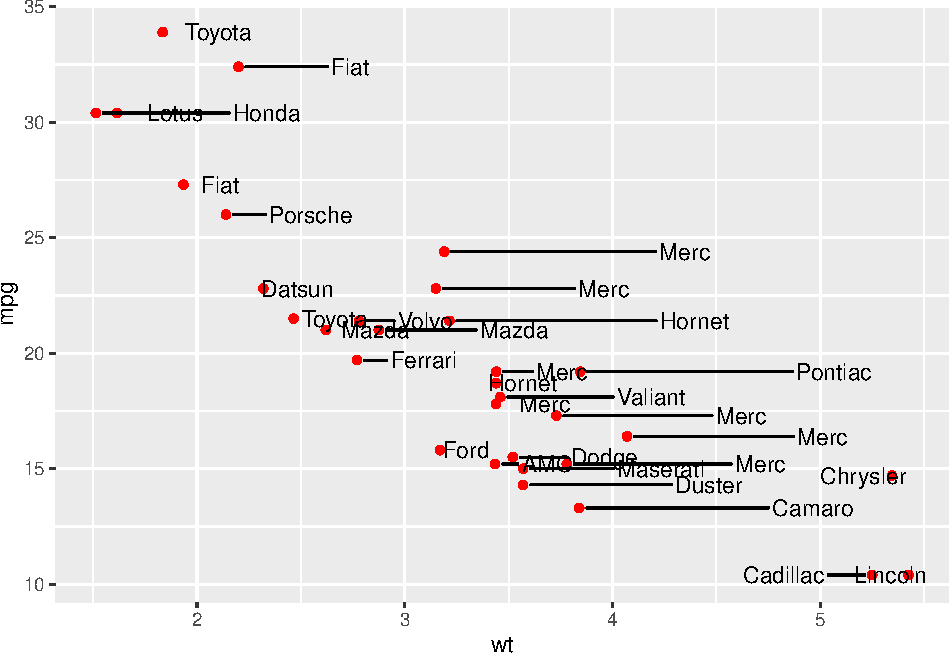
\includegraphics{TRES-Tidy-Tutorial_files/figure-latex/unnamed-chunk-27-1.pdf}

This is not a good looking plot, because it breaks other rules of plot design, such as whether this sort of plot should be made at all. Labels and text need to be applied sparingly, for example drawing attention or adding information to outliers.

\hypertarget{reshaping-data-tables-in-the-tidyverse}{%
\chapter{Reshaping data tables in the tidyverse}\label{reshaping-data-tables-in-the-tidyverse}}

Raphael Scherrer


\includegraphics{opening-image.png}

\begin{Shaded}
\begin{Highlighting}[]
\KeywordTok{library}\NormalTok{(tibble)}
\KeywordTok{library}\NormalTok{(tidyr)}
\end{Highlighting}
\end{Shaded}

In this chapter we will learn what \emph{tidy} means in the context of the tidyverse, and how to reshape our data into a tidy format using the \texttt{tidyr} package. But first, let us take a detour and introduce the \texttt{tibble}.

\hypertarget{the-new-data-frame-tibble}{%
\section{1. The new data frame: tibble}\label{the-new-data-frame-tibble}}

The \texttt{tibble} is the recommended class to use to store tabular data in the tidyverse. Consider it as the operational unit of any data science pipeline. For most practical purposes, a \texttt{tibble} is basically a \texttt{data.frame}.

\begin{Shaded}
\begin{Highlighting}[]
\CommentTok{# Make a data frame}
\KeywordTok{data.frame}\NormalTok{(}\DataTypeTok{who =} \KeywordTok{c}\NormalTok{(}\StringTok{"Pratik"}\NormalTok{, }\StringTok{"Theo"}\NormalTok{, }\StringTok{"Raph"}\NormalTok{), }\DataTypeTok{chapt =} \KeywordTok{c}\NormalTok{(}\StringTok{"1, 4"}\NormalTok{, }\StringTok{"3"}\NormalTok{, }\StringTok{"2, 5"}\NormalTok{))}
\end{Highlighting}
\end{Shaded}

\begin{verbatim}
##      who chapt
## 1 Pratik  1, 4
## 2   Theo     3
## 3   Raph  2, 5
\end{verbatim}

\begin{Shaded}
\begin{Highlighting}[]
\CommentTok{# Or an equivalent tibble}
\KeywordTok{tibble}\NormalTok{(}\DataTypeTok{who =} \KeywordTok{c}\NormalTok{(}\StringTok{"Pratik"}\NormalTok{, }\StringTok{"Theo"}\NormalTok{, }\StringTok{"Raph"}\NormalTok{), }\DataTypeTok{chapt =} \KeywordTok{c}\NormalTok{(}\StringTok{"1, 4"}\NormalTok{, }\StringTok{"3"}\NormalTok{, }\StringTok{"2, 5"}\NormalTok{))}
\end{Highlighting}
\end{Shaded}

\begin{verbatim}
## # A tibble: 3 x 2
##   who    chapt
##   <chr>  <chr>
## 1 Pratik 1, 4 
## 2 Theo   3    
## 3 Raph   2, 5
\end{verbatim}

The difference between \texttt{tibble} and \texttt{data.frame} is in its display and in the way it is subsetted, among others. Most functions working with \texttt{data.frame} will work with \texttt{tibble} and vice versa. Use the \texttt{as*} family of functions to switch back and forth between the two if needed, using e.g.~\texttt{as.data.frame} or \texttt{as\_tibble}.

In terms of display, the tibble has the advantage of showing the class of each column: \texttt{chr} for \texttt{character}, \texttt{fct} for \texttt{factor}, \texttt{int} for \texttt{integer}, \texttt{dbl} for \texttt{numeric} and \texttt{lgl} for \texttt{logical}, just to name the main atomic classes. This may be more important than you think, because many hard-to-find bugs in R are due to wrong variable types and/or cryptic type conversions. This especially happens with \texttt{factor} and \texttt{character}, which can cause quite some confusion. More about this in the extra section at the end of this chapter!

Note that you can build a tibble by rows rather than by columns with \texttt{tribble}:

\begin{Shaded}
\begin{Highlighting}[]
\KeywordTok{tribble}\NormalTok{(}
  \OperatorTok{~}\NormalTok{who, }\OperatorTok{~}\NormalTok{chapt,}
  \StringTok{"Pratik"}\NormalTok{, }\StringTok{"1, 4"}\NormalTok{,}
  \StringTok{"Theo"}\NormalTok{, }\StringTok{"3"}\NormalTok{,}
  \StringTok{"Raph"}\NormalTok{, }\StringTok{"2, 5"}
\NormalTok{)}
\end{Highlighting}
\end{Shaded}

\begin{verbatim}
## # A tibble: 3 x 2
##   who    chapt
##   <chr>  <chr>
## 1 Pratik 1, 4 
## 2 Theo   3    
## 3 Raph   2, 5
\end{verbatim}

As a rule of thumb, try to convert your tables to tibbles whenever you can, especially when the original table is \emph{not} a data frame. For example, the principal component analysis function \texttt{prcomp} outputs a \texttt{matrix} of coordinates in principal component-space.

\begin{Shaded}
\begin{Highlighting}[]
\CommentTok{# Perform a PCA on mtcars }
\NormalTok{pca_scores <-}\StringTok{ }\KeywordTok{prcomp}\NormalTok{(mtcars)}\OperatorTok{$}\NormalTok{x}
\KeywordTok{head}\NormalTok{(pca_scores) }\CommentTok{# looks like a data frame or a tibble...}
\end{Highlighting}
\end{Shaded}

\begin{verbatim}
##                           PC1       PC2       PC3        PC4        PC5
## Mazda RX4          -79.596425  2.132241 -2.153336 -2.7073437 -0.7023522
## Mazda RX4 Wag      -79.598570  2.147487 -2.215124 -2.1782888 -0.8843859
## Datsun 710        -133.894096 -5.057570 -2.137950  0.3460330  1.1061111
## Hornet 4 Drive       8.516559 44.985630  1.233763  0.8273631  0.4240145
## Hornet Sportabout  128.686342 30.817402  3.343421 -0.5211000  0.7365801
## Valiant            -23.220146 35.106518 -3.259562  1.4005360  0.8029768
##                           PC6          PC7         PC8        PC9        PC10
## Mazda RX4         -0.31486106 -0.098695018 -0.07789812 -0.2000092 -0.29008191
## Mazda RX4 Wag     -0.45343873 -0.003554594 -0.09566630 -0.3533243 -0.19283553
## Datsun 710         1.17298584  0.005755581  0.13624782 -0.1976423  0.07634353
## Hornet 4 Drive    -0.05789705 -0.024307168  0.22120800  0.3559844 -0.09057039
## Hornet Sportabout -0.33290957  0.106304777 -0.05301719  0.1532714 -0.18862217
## Valiant           -0.08837864  0.238946304  0.42390551  0.1012944 -0.03769010
##                         PC11
## Mazda RX4          0.1057706
## Mazda RX4 Wag      0.1069047
## Datsun 710         0.2668713
## Hornet 4 Drive     0.2088354
## Hornet Sportabout -0.1092563
## Valiant            0.2757693
\end{verbatim}

\begin{Shaded}
\begin{Highlighting}[]
\KeywordTok{class}\NormalTok{(pca_scores) }\CommentTok{# but is actually a matrix}
\end{Highlighting}
\end{Shaded}

\begin{verbatim}
## [1] "matrix"
\end{verbatim}

\begin{Shaded}
\begin{Highlighting}[]
\CommentTok{# Convert to tibble}
\KeywordTok{as_tibble}\NormalTok{(pca_scores)}
\end{Highlighting}
\end{Shaded}

\begin{verbatim}
## # A tibble: 32 x 11
##        PC1    PC2    PC3    PC4    PC5     PC6      PC7     PC8    PC9    PC10
##      <dbl>  <dbl>  <dbl>  <dbl>  <dbl>   <dbl>    <dbl>   <dbl>  <dbl>   <dbl>
##  1  -79.6    2.13 -2.15  -2.71  -0.702 -0.315  -0.0987  -0.0779 -0.200 -0.290 
##  2  -79.6    2.15 -2.22  -2.18  -0.884 -0.453  -0.00355 -0.0957 -0.353 -0.193 
##  3 -134.    -5.06 -2.14   0.346  1.11   1.17    0.00576  0.136  -0.198  0.0763
##  4    8.52  45.0   1.23   0.827  0.424 -0.0579 -0.0243   0.221   0.356 -0.0906
##  5  129.    30.8   3.34  -0.521  0.737 -0.333   0.106   -0.0530  0.153 -0.189 
##  6  -23.2   35.1  -3.26   1.40   0.803 -0.0884  0.239    0.424   0.101 -0.0377
##  7  159.   -32.3   0.649  0.199  0.786  0.0687 -0.530   -0.0593  0.221 -0.313 
##  8 -113.    39.7  -0.465  0.338 -1.24   0.280  -0.146    0.320   0.279  0.190 
##  9 -104.     7.51 -1.59   4.02  -1.14   0.0279  0.595   -0.233  -0.126 -0.349 
## 10  -67.0   -6.21 -3.61  -0.320 -0.960 -0.529  -0.0174  -0.182   0.543  0.412 
## # ... with 22 more rows, and 1 more variable: PC11 <dbl>
\end{verbatim}

This is important because a \texttt{matrix} can contain only one type of values (e.g.~only \texttt{numeric} or \texttt{character}), while \texttt{tibble} (and \texttt{data.frame}) allow you to have columns of different types.

So, in the tidyverse we are going to work with tibbles, got it. But what does ``tidy'' mean exactly?

\hypertarget{the-concept-of-tidy-data}{%
\section{2. The concept of tidy data}\label{the-concept-of-tidy-data}}

When it comes to putting data into tables, there are many ways one could organize a dataset. The \emph{tidy} format is one such format. According to the formal \href{https://tidyr.tidyverse.org/articles/tidy-data.html}{definition}, a table is tidy if each column is a variable and each row is an observation. In practice, however, I found that this is not a very operational definition, especially in ecology and evolution where we often record multiple variables per individual. So, let's dig in with an example.

Say we have a dataset of several morphometrics measured on Darwin's finches in the Galapagos islands. Let's first get this dataset.

\begin{Shaded}
\begin{Highlighting}[]
\CommentTok{# We first simulate random data}
\NormalTok{beak_lengths <-}\StringTok{ }\KeywordTok{rnorm}\NormalTok{(}\DecValTok{100}\NormalTok{, }\DataTypeTok{mean =} \DecValTok{5}\NormalTok{, }\DataTypeTok{sd =} \FloatTok{0.1}\NormalTok{)}
\NormalTok{beak_widths <-}\StringTok{ }\KeywordTok{rnorm}\NormalTok{(}\DecValTok{100}\NormalTok{, }\DataTypeTok{mean =} \DecValTok{2}\NormalTok{, }\DataTypeTok{sd =} \FloatTok{0.1}\NormalTok{)}
\NormalTok{body_weights <-}\StringTok{ }\KeywordTok{rgamma}\NormalTok{(}\DecValTok{100}\NormalTok{, }\DataTypeTok{shape =} \DecValTok{10}\NormalTok{, }\DataTypeTok{rate =} \DecValTok{1}\NormalTok{)}
\NormalTok{islands <-}\StringTok{ }\KeywordTok{rep}\NormalTok{(}\KeywordTok{c}\NormalTok{(}\StringTok{"Isabela"}\NormalTok{, }\StringTok{"Santa Cruz"}\NormalTok{), }\DataTypeTok{each =} \DecValTok{50}\NormalTok{)}

\CommentTok{# Assemble into a tibble}
\NormalTok{data <-}\StringTok{ }\KeywordTok{tibble}\NormalTok{(}
  \DataTypeTok{id =} \DecValTok{1}\OperatorTok{:}\DecValTok{100}\NormalTok{,}
  \DataTypeTok{beak_length =}\NormalTok{ beak_lengths, }
  \DataTypeTok{beak_width =}\NormalTok{ beak_widths, }
  \DataTypeTok{body_weight =}\NormalTok{ body_weights,}
  \DataTypeTok{island =}\NormalTok{ islands}
\NormalTok{)}

\CommentTok{# Snapshot}
\NormalTok{data}
\end{Highlighting}
\end{Shaded}

\begin{verbatim}
## # A tibble: 100 x 5
##       id beak_length beak_width body_weight island 
##    <int>       <dbl>      <dbl>       <dbl> <chr>  
##  1     1        4.99       2.05        9.23 Isabela
##  2     2        4.97       2.22        6.75 Isabela
##  3     3        5.08       1.91        7.14 Isabela
##  4     4        5.07       1.97        8.70 Isabela
##  5     5        4.90       2.10       10.2  Isabela
##  6     6        5.08       2.03       10.3  Isabela
##  7     7        4.98       1.87        8.16 Isabela
##  8     8        5.06       2.08       10.5  Isabela
##  9     9        4.94       2.08       10.4  Isabela
## 10    10        4.87       1.92        8.62 Isabela
## # ... with 90 more rows
\end{verbatim}

Here, we pretend to have measured \texttt{beak\_length}, \texttt{beak\_width} and \texttt{body\_weight} on 100 birds, 50 of them from Isabela and 50 of them from Santa Cruz. In this tibble, each row is an individual bird. This is probably the way most scientists would record their data in the field. However, a single bird is not an ``observation'' in the sense used in the tidyverse. Our dataset is not tidy but \emph{messy}.

The tidy equivalent of this dataset would be:

\begin{Shaded}
\begin{Highlighting}[]
\NormalTok{data <-}\StringTok{ }\KeywordTok{pivot_longer}\NormalTok{(}
\NormalTok{  data, }
  \DataTypeTok{cols =} \KeywordTok{c}\NormalTok{(}\StringTok{"beak_length"}\NormalTok{, }\StringTok{"beak_width"}\NormalTok{, }\StringTok{"body_weight"}\NormalTok{),}
  \DataTypeTok{names_to =} \StringTok{"variable"}
\NormalTok{)}
\NormalTok{data}
\end{Highlighting}
\end{Shaded}

\begin{verbatim}
## # A tibble: 300 x 4
##       id island  variable    value
##    <int> <chr>   <chr>       <dbl>
##  1     1 Isabela beak_length  4.99
##  2     1 Isabela beak_width   2.05
##  3     1 Isabela body_weight  9.23
##  4     2 Isabela beak_length  4.97
##  5     2 Isabela beak_width   2.22
##  6     2 Isabela body_weight  6.75
##  7     3 Isabela beak_length  5.08
##  8     3 Isabela beak_width   1.91
##  9     3 Isabela body_weight  7.14
## 10     4 Isabela beak_length  5.07
## # ... with 290 more rows
\end{verbatim}

where each \emph{measurement} (and not each \emph{individual}) is now the unit of observation (the rows). We will come back to the \texttt{pivot\_longer} function later.

As you can see our tibble now has three times as many rows and fewer columns. This format is rather unintuitive and not optimal for display. However, it provides a very standardized and consistent way of organizing data that will be understood (and expected) by pretty much all functions in the tidyverse. This makes the tidyverse tools work well together and reduces the time you would otherwise spend reformatting your data from one tool to the next.

That does not mean that the \emph{messy} format is useless though. There may be use-cases where you need to switch back and forth between formats. For this reason I prefer referring to these formats using their other names: \emph{long} (tidy) versus \emph{wide} (messy). For example, matrix operations work much faster on wide data, and the wide format arguably looks nicer for display. Luckily the \texttt{tidyr} package gives us the tools to reshape our data as needed, as we shall see shortly.

Another common example of wide-or-long dilemma is when dealing with \emph{contingency tables}. This would be our case, for example, if we asked how many observations we have for each morphometric and each island. We use \texttt{table} (from base R) to get the answer:

\begin{Shaded}
\begin{Highlighting}[]
\CommentTok{# Make a contingency table}
\NormalTok{ctg <-}\StringTok{ }\KeywordTok{with}\NormalTok{(data, }\KeywordTok{table}\NormalTok{(island, variable))}
\NormalTok{ctg}
\end{Highlighting}
\end{Shaded}

\begin{verbatim}
##             variable
## island       beak_length beak_width body_weight
##   Isabela             50         50          50
##   Santa Cruz          50         50          50
\end{verbatim}

A variety of statistical tests can be used on contingency tables such as Fisher's exact test, the chi-square test or the binomial test. Contingency tables are in the wide format by construction, but they too can be pivoted to the long format, and the tidyverse manipulation tools will expect you to do so. Actually, \texttt{tibble} knows that very well and does it by default if you convert your \texttt{table} into a \texttt{tibble}:

\begin{Shaded}
\begin{Highlighting}[]
\CommentTok{# Contingency table is pivoted to the long-format automatically}
\KeywordTok{as_tibble}\NormalTok{(ctg)}
\end{Highlighting}
\end{Shaded}

\begin{verbatim}
## # A tibble: 6 x 3
##   island     variable        n
##   <chr>      <chr>       <int>
## 1 Isabela    beak_length    50
## 2 Santa Cruz beak_length    50
## 3 Isabela    beak_width     50
## 4 Santa Cruz beak_width     50
## 5 Isabela    body_weight    50
## 6 Santa Cruz body_weight    50
\end{verbatim}

\hypertarget{reshaping-with-tidyr}{%
\section{\texorpdfstring{3. Reshaping with \texttt{tidyr}}{3. Reshaping with tidyr}}\label{reshaping-with-tidyr}}

The \texttt{tidyr} package implements tools to easily switch between layouts and also perform a few other reshaping operations. Old school R users will be familiar with the \texttt{reshape} and \texttt{reshape2} packages, of which \texttt{tidyr} is the tidyverse equivalent. Beware that \texttt{tidyr} is about playing with the general \emph{layout} of the dataset, while \emph{operations} and \emph{transformations} of the data are within the scope of the \texttt{dplyr} and \texttt{purrr} packages. All these packages work hand-in-hand really well, and analysis pipelines usually involve all of them. But today, we focus on the first member of this holy trinity, which is often the first one you'll need because you will want to reshape your data before doing other things. So, please hold your non-layout-related questions for the next chapters.

\hypertarget{pivoting}{%
\subsection{3.1. Pivoting}\label{pivoting}}

Pivoting a dataset between the long and wide layout is the main purpose of \texttt{tidyr} (check out the package's logo). We already saw the \texttt{pivot\_longer} function, that converts a table form wide to long format. Similarly, there is a \texttt{pivot\_wider} function that does exactly the opposite and takes you back to the wide format:

\begin{Shaded}
\begin{Highlighting}[]
\KeywordTok{pivot_wider}\NormalTok{(}
\NormalTok{  data, }
  \DataTypeTok{names_from =} \StringTok{"variable"}\NormalTok{, }
  \DataTypeTok{values_from =} \StringTok{"value"}\NormalTok{, }
  \DataTypeTok{id_cols =} \KeywordTok{c}\NormalTok{(}\StringTok{"id"}\NormalTok{, }\StringTok{"island"}\NormalTok{)}
\NormalTok{)}
\end{Highlighting}
\end{Shaded}

\begin{verbatim}
## # A tibble: 100 x 5
##       id island  beak_length beak_width body_weight
##    <int> <chr>         <dbl>      <dbl>       <dbl>
##  1     1 Isabela        4.99       2.05        9.23
##  2     2 Isabela        4.97       2.22        6.75
##  3     3 Isabela        5.08       1.91        7.14
##  4     4 Isabela        5.07       1.97        8.70
##  5     5 Isabela        4.90       2.10       10.2 
##  6     6 Isabela        5.08       2.03       10.3 
##  7     7 Isabela        4.98       1.87        8.16
##  8     8 Isabela        5.06       2.08       10.5 
##  9     9 Isabela        4.94       2.08       10.4 
## 10    10 Isabela        4.87       1.92        8.62
## # ... with 90 more rows
\end{verbatim}

The order of the columns is not exactly as it was, but this should not matter in a data analysis pipeline where you should access columns by their names. It is straightforward to change the order of the columns, but this is more within the scope of the \texttt{dplyr} package.

If you are familiar with earlier versions of the tidyverse, \texttt{pivot\_longer} and \texttt{pivot\_wider} are the respective equivalents of \texttt{gather} and \texttt{spread}, which are now deprecated.

There are a few other reshaping operations from \texttt{tidyr} that are worth knowing.

\hypertarget{handling-missing-values}{%
\subsection{3.2. Handling missing values}\label{handling-missing-values}}

Say we have some missing measurements in the column ``value'' of our finch dataset:

\begin{Shaded}
\begin{Highlighting}[]
\CommentTok{# We replace 100 random observations by NAs}
\NormalTok{ii <-}\StringTok{ }\KeywordTok{sample}\NormalTok{(}\KeywordTok{nrow}\NormalTok{(data), }\DecValTok{100}\NormalTok{)}
\NormalTok{data}\OperatorTok{$}\NormalTok{value[ii] <-}\StringTok{ }\OtherTok{NA}
\NormalTok{data}
\end{Highlighting}
\end{Shaded}

\begin{verbatim}
## # A tibble: 300 x 4
##       id island  variable    value
##    <int> <chr>   <chr>       <dbl>
##  1     1 Isabela beak_length  4.99
##  2     1 Isabela beak_width   2.05
##  3     1 Isabela body_weight  9.23
##  4     2 Isabela beak_length  4.97
##  5     2 Isabela beak_width   2.22
##  6     2 Isabela body_weight  6.75
##  7     3 Isabela beak_length NA   
##  8     3 Isabela beak_width   1.91
##  9     3 Isabela body_weight NA   
## 10     4 Isabela beak_length  5.07
## # ... with 290 more rows
\end{verbatim}

We could get rid of the rows that have missing values using \texttt{drop\_na}:

\begin{Shaded}
\begin{Highlighting}[]
\KeywordTok{drop_na}\NormalTok{(data, value)}
\end{Highlighting}
\end{Shaded}

\begin{verbatim}
## # A tibble: 200 x 4
##       id island  variable    value
##    <int> <chr>   <chr>       <dbl>
##  1     1 Isabela beak_length  4.99
##  2     1 Isabela beak_width   2.05
##  3     1 Isabela body_weight  9.23
##  4     2 Isabela beak_length  4.97
##  5     2 Isabela beak_width   2.22
##  6     2 Isabela body_weight  6.75
##  7     3 Isabela beak_width   1.91
##  8     4 Isabela beak_length  5.07
##  9     5 Isabela beak_length  4.90
## 10     5 Isabela beak_width   2.10
## # ... with 190 more rows
\end{verbatim}

Else, we could replace the NAs with some user-defined value:

\begin{Shaded}
\begin{Highlighting}[]
\KeywordTok{replace_na}\NormalTok{(data, }\DataTypeTok{replace =} \KeywordTok{list}\NormalTok{(}\DataTypeTok{value =} \DecValTok{-999}\NormalTok{))}
\end{Highlighting}
\end{Shaded}

\begin{verbatim}
## # A tibble: 300 x 4
##       id island  variable      value
##    <int> <chr>   <chr>         <dbl>
##  1     1 Isabela beak_length    4.99
##  2     1 Isabela beak_width     2.05
##  3     1 Isabela body_weight    9.23
##  4     2 Isabela beak_length    4.97
##  5     2 Isabela beak_width     2.22
##  6     2 Isabela body_weight    6.75
##  7     3 Isabela beak_length -999   
##  8     3 Isabela beak_width     1.91
##  9     3 Isabela body_weight -999   
## 10     4 Isabela beak_length    5.07
## # ... with 290 more rows
\end{verbatim}

where the \texttt{replace} argument takes a named list, and the names should refer to the columns to apply the replacement to.

We could also replace NAs with the most recent non-NA values:

\begin{Shaded}
\begin{Highlighting}[]
\KeywordTok{fill}\NormalTok{(data, value)}
\end{Highlighting}
\end{Shaded}

\begin{verbatim}
## # A tibble: 300 x 4
##       id island  variable    value
##    <int> <chr>   <chr>       <dbl>
##  1     1 Isabela beak_length  4.99
##  2     1 Isabela beak_width   2.05
##  3     1 Isabela body_weight  9.23
##  4     2 Isabela beak_length  4.97
##  5     2 Isabela beak_width   2.22
##  6     2 Isabela body_weight  6.75
##  7     3 Isabela beak_length  6.75
##  8     3 Isabela beak_width   1.91
##  9     3 Isabela body_weight  1.91
## 10     4 Isabela beak_length  5.07
## # ... with 290 more rows
\end{verbatim}

Note that most functions in the tidyverse take a tibble as their first argument, and columns to which to apply the functions are usually passed as ``objects'' rather than character strings. In the above example, we passed the \texttt{value} column as \texttt{value}, not \texttt{"value"}. These column-objects are called by the tidyverse functions \emph{in the context} of the data (the tibble) they belong to.

\hypertarget{splitting-and-combining-cells}{%
\subsection{3.3. Splitting and combining cells}\label{splitting-and-combining-cells}}

The \texttt{tidyr} package offers tools to split and combine columns. This is a nice extension to the string manipulations we saw last week in the \texttt{stringr} tutorial.

Say we want to add the specific dates when we took measurements on our birds (we would normally do this using \texttt{dplyr} but for now we will stick to the old way):

\begin{Shaded}
\begin{Highlighting}[]
\CommentTok{# Sample random dates for each observation}
\NormalTok{data}\OperatorTok{$}\NormalTok{day <-}\StringTok{ }\KeywordTok{sample}\NormalTok{(}\DecValTok{30}\NormalTok{, }\KeywordTok{nrow}\NormalTok{(data), }\DataTypeTok{replace =} \OtherTok{TRUE}\NormalTok{)}
\NormalTok{data}\OperatorTok{$}\NormalTok{month <-}\StringTok{ }\KeywordTok{sample}\NormalTok{(}\DecValTok{12}\NormalTok{, }\KeywordTok{nrow}\NormalTok{(data), }\DataTypeTok{replace =} \OtherTok{TRUE}\NormalTok{)}
\NormalTok{data}\OperatorTok{$}\NormalTok{year <-}\StringTok{ }\KeywordTok{sample}\NormalTok{(}\DecValTok{2019}\OperatorTok{:}\DecValTok{2020}\NormalTok{, }\KeywordTok{nrow}\NormalTok{(data), }\DataTypeTok{replace =} \OtherTok{TRUE}\NormalTok{)}
\NormalTok{data}
\end{Highlighting}
\end{Shaded}

\begin{verbatim}
## # A tibble: 300 x 7
##       id island  variable    value   day month  year
##    <int> <chr>   <chr>       <dbl> <int> <int> <int>
##  1     1 Isabela beak_length  4.99    22     3  2020
##  2     1 Isabela beak_width   2.05    17     7  2019
##  3     1 Isabela body_weight  9.23     1    10  2020
##  4     2 Isabela beak_length  4.97     9     2  2020
##  5     2 Isabela beak_width   2.22    23     1  2020
##  6     2 Isabela body_weight  6.75    15     2  2020
##  7     3 Isabela beak_length NA       12     2  2020
##  8     3 Isabela beak_width   1.91    22    12  2019
##  9     3 Isabela body_weight NA       23     9  2019
## 10     4 Isabela beak_length  5.07     8     9  2020
## # ... with 290 more rows
\end{verbatim}

We could combine the \texttt{day}, \texttt{month} and \texttt{year} columns into a single \texttt{date} column, with a dash as a separator, using \texttt{unite}:

\begin{Shaded}
\begin{Highlighting}[]
\NormalTok{data <-}\StringTok{ }\KeywordTok{unite}\NormalTok{(data, day, month, year, }\DataTypeTok{col =} \StringTok{"date"}\NormalTok{, }\DataTypeTok{sep =} \StringTok{"-"}\NormalTok{)}
\NormalTok{data}
\end{Highlighting}
\end{Shaded}

\begin{verbatim}
## # A tibble: 300 x 5
##       id island  variable    value date      
##    <int> <chr>   <chr>       <dbl> <chr>     
##  1     1 Isabela beak_length  4.99 22-3-2020 
##  2     1 Isabela beak_width   2.05 17-7-2019 
##  3     1 Isabela body_weight  9.23 1-10-2020 
##  4     2 Isabela beak_length  4.97 9-2-2020  
##  5     2 Isabela beak_width   2.22 23-1-2020 
##  6     2 Isabela body_weight  6.75 15-2-2020 
##  7     3 Isabela beak_length NA    12-2-2020 
##  8     3 Isabela beak_width   1.91 22-12-2019
##  9     3 Isabela body_weight NA    23-9-2019 
## 10     4 Isabela beak_length  5.07 8-9-2020  
## # ... with 290 more rows
\end{verbatim}

Of course, we can revert back to the previous dataset by splitting the \texttt{date} column with \texttt{separate}.

\begin{Shaded}
\begin{Highlighting}[]
\KeywordTok{separate}\NormalTok{(data, date, }\DataTypeTok{into =} \KeywordTok{c}\NormalTok{(}\StringTok{"day"}\NormalTok{, }\StringTok{"month"}\NormalTok{, }\StringTok{"year"}\NormalTok{))}
\end{Highlighting}
\end{Shaded}

\begin{verbatim}
## # A tibble: 300 x 7
##       id island  variable    value day   month year 
##    <int> <chr>   <chr>       <dbl> <chr> <chr> <chr>
##  1     1 Isabela beak_length  4.99 22    3     2020 
##  2     1 Isabela beak_width   2.05 17    7     2019 
##  3     1 Isabela body_weight  9.23 1     10    2020 
##  4     2 Isabela beak_length  4.97 9     2     2020 
##  5     2 Isabela beak_width   2.22 23    1     2020 
##  6     2 Isabela body_weight  6.75 15    2     2020 
##  7     3 Isabela beak_length NA    12    2     2020 
##  8     3 Isabela beak_width   1.91 22    12    2019 
##  9     3 Isabela body_weight NA    23    9     2019 
## 10     4 Isabela beak_length  5.07 8     9     2020 
## # ... with 290 more rows
\end{verbatim}

But note that the \texttt{day}, \texttt{month} and \texttt{year} columns are now of class \texttt{character} and not \texttt{integer} anymore. This is because they result from the splitting of \texttt{date}, which itself was a \texttt{character} column.

You can also separate a single column into multiple \emph{rows} using \texttt{separate\_rows}:

\begin{Shaded}
\begin{Highlighting}[]
\KeywordTok{separate_rows}\NormalTok{(data, date)}
\end{Highlighting}
\end{Shaded}

\begin{verbatim}
## # A tibble: 900 x 5
##       id island  variable    value date 
##    <int> <chr>   <chr>       <dbl> <chr>
##  1     1 Isabela beak_length  4.99 22   
##  2     1 Isabela beak_length  4.99 3    
##  3     1 Isabela beak_length  4.99 2020 
##  4     1 Isabela beak_width   2.05 17   
##  5     1 Isabela beak_width   2.05 7    
##  6     1 Isabela beak_width   2.05 2019 
##  7     1 Isabela body_weight  9.23 1    
##  8     1 Isabela body_weight  9.23 10   
##  9     1 Isabela body_weight  9.23 2020 
## 10     2 Isabela beak_length  4.97 9    
## # ... with 890 more rows
\end{verbatim}

\hypertarget{expanding-tables-using-combinations}{%
\subsection{3.4. Expanding tables using combinations}\label{expanding-tables-using-combinations}}

Sometimes one may need to quickly create a table with all combinations of a set of variables. We could generate a tibble with all combinations of island-by-morphometric using \texttt{expand\_grid}:

\begin{Shaded}
\begin{Highlighting}[]
\KeywordTok{expand_grid}\NormalTok{(}
  \DataTypeTok{island =} \KeywordTok{c}\NormalTok{(}\StringTok{"Isabela"}\NormalTok{, }\StringTok{"Santa Cruz"}\NormalTok{), }
  \DataTypeTok{variable =} \KeywordTok{c}\NormalTok{(}\StringTok{"beak_length"}\NormalTok{, }\StringTok{"beak_width"}\NormalTok{, }\StringTok{"body_weight"}\NormalTok{)}
\NormalTok{)}
\end{Highlighting}
\end{Shaded}

\begin{verbatim}
## # A tibble: 6 x 2
##   island     variable   
##   <chr>      <chr>      
## 1 Isabela    beak_length
## 2 Isabela    beak_width 
## 3 Isabela    body_weight
## 4 Santa Cruz beak_length
## 5 Santa Cruz beak_width 
## 6 Santa Cruz body_weight
\end{verbatim}

If we already have a tibble to work from that contains the variables to combine, we can use \texttt{expand}:

\begin{Shaded}
\begin{Highlighting}[]
\KeywordTok{expand}\NormalTok{(data, island, variable)}
\end{Highlighting}
\end{Shaded}

\begin{verbatim}
## # A tibble: 6 x 2
##   island     variable   
##   <chr>      <chr>      
## 1 Isabela    beak_length
## 2 Isabela    beak_width 
## 3 Isabela    body_weight
## 4 Santa Cruz beak_length
## 5 Santa Cruz beak_width 
## 6 Santa Cruz body_weight
\end{verbatim}

As an extension of this, the function \texttt{complete} can come particularly handy if we need to add missing combinations to our tibble:

\begin{Shaded}
\begin{Highlighting}[]
\KeywordTok{complete}\NormalTok{(data, island, variable)}
\end{Highlighting}
\end{Shaded}

\begin{verbatim}
## # A tibble: 300 x 5
##    island  variable       id value date     
##    <chr>   <chr>       <int> <dbl> <chr>    
##  1 Isabela beak_length     1  4.99 22-3-2020
##  2 Isabela beak_length     2  4.97 9-2-2020 
##  3 Isabela beak_length     3 NA    12-2-2020
##  4 Isabela beak_length     4  5.07 8-9-2020 
##  5 Isabela beak_length     5  4.90 26-3-2019
##  6 Isabela beak_length     6  5.08 17-9-2020
##  7 Isabela beak_length     7 NA    17-6-2020
##  8 Isabela beak_length     8  5.06 2-10-2020
##  9 Isabela beak_length     9 NA    21-9-2020
## 10 Isabela beak_length    10  4.87 7-5-2020 
## # ... with 290 more rows
\end{verbatim}

which does nothing here because we already have all combinations of \texttt{island} and \texttt{variable}.

\hypertarget{nesting}{%
\subsection{3.5. Nesting}\label{nesting}}

The \texttt{tidyr} package has yet another feature that makes the tidyverse very powerful: the \texttt{nest} function. However, it makes little sense without combining it with the functions in the \texttt{purrr} package, so we will not cover it in this chapter but rather in the \texttt{purrr} chapter.

\hypertarget{extra-factors-and-the-forcats-package}{%
\section{\texorpdfstring{4. Extra: factors and the \texttt{forcats} package}{4. Extra: factors and the forcats package}}\label{extra-factors-and-the-forcats-package}}

\begin{Shaded}
\begin{Highlighting}[]
\KeywordTok{library}\NormalTok{(forcats)}
\end{Highlighting}
\end{Shaded}

Categorical variables can be stored in R as character strings in \texttt{character} or \texttt{factor} objects. A \texttt{factor} looks like a \texttt{character}, but it actually is an \texttt{integer} vector, where each \texttt{integer} is mapped to a \texttt{character} label. With this respect it is sort of an enhanced version of \texttt{character}. For example,

\begin{Shaded}
\begin{Highlighting}[]
\NormalTok{my_char_vec <-}\StringTok{ }\KeywordTok{c}\NormalTok{(}\StringTok{"Pratik"}\NormalTok{, }\StringTok{"Theo"}\NormalTok{, }\StringTok{"Raph"}\NormalTok{)}
\NormalTok{my_char_vec}
\end{Highlighting}
\end{Shaded}

\begin{verbatim}
## [1] "Pratik" "Theo"   "Raph"
\end{verbatim}

is a \texttt{character} vector, recognizable to its double quotes, while

\begin{Shaded}
\begin{Highlighting}[]
\NormalTok{my_fact_vec <-}\StringTok{ }\KeywordTok{factor}\NormalTok{(my_char_vec) }\CommentTok{# as.factor would work too}
\NormalTok{my_fact_vec}
\end{Highlighting}
\end{Shaded}

\begin{verbatim}
## [1] Pratik Theo   Raph  
## Levels: Pratik Raph Theo
\end{verbatim}

is a \texttt{factor}, of which the \emph{labels} are displayed. The \emph{levels} of the factor are the unique values that appear in the vector. If I added an extra occurrence of my name:

\begin{Shaded}
\begin{Highlighting}[]
\KeywordTok{factor}\NormalTok{(}\KeywordTok{c}\NormalTok{(my_char_vec, }\StringTok{"Raph"}\NormalTok{))}
\end{Highlighting}
\end{Shaded}

\begin{verbatim}
## [1] Pratik Theo   Raph   Raph  
## Levels: Pratik Raph Theo
\end{verbatim}

we would still have the the same levels. Note that the levels are returned as a \texttt{character} vector in alphabetical order by the \texttt{levels} function:

\begin{Shaded}
\begin{Highlighting}[]
\KeywordTok{levels}\NormalTok{(my_fact_vec)}
\end{Highlighting}
\end{Shaded}

\begin{verbatim}
## [1] "Pratik" "Raph"   "Theo"
\end{verbatim}

Why does it matter? Well, most operations on categorical variables can be performed on \texttt{character} of \texttt{factor} objects, so it does not matter so much which one you use for your own data. However, some functions in R require you to provide categorical variables in one specific format, and others may even implicitely convert your variables. In \texttt{ggplot2} for example, character vectors are converted into factors by default. So, it is always good to remember the differences and what type your variables are.

But this is a tidyverse tutorial, so I would like to introduce here the package \texttt{forcats}, which offers tools to manipulate factors. First of all, most tools from \texttt{stringr} \emph{will work} on factors. The \texttt{forcats} functions expand the string manipulation toolbox with factor-specific utilities. Similar in philosophy to \texttt{stringr} where functions started with \texttt{str\_}, in \texttt{forcats} most functions start with \texttt{fct\_}.

I see two main ways \texttt{forcats} can come handy in the kind of data most people deal with: playing with the order of the levels of a factor and playing with the levels themselves. We will show here a few examples, but the full breadth of factor manipulations can be found online or in the excellent \texttt{forcats} cheatsheet.

\hypertarget{reordering-a-factor}{%
\subsection{4.1. Reordering a factor}\label{reordering-a-factor}}

Use \texttt{fct\_relevel} to manually change the order of the levels:

\begin{Shaded}
\begin{Highlighting}[]
\KeywordTok{fct_relevel}\NormalTok{(my_fact_vec, }\KeywordTok{c}\NormalTok{(}\StringTok{"Pratik"}\NormalTok{, }\StringTok{"Theo"}\NormalTok{, }\StringTok{"Raph"}\NormalTok{))}
\end{Highlighting}
\end{Shaded}

\begin{verbatim}
## [1] Pratik Theo   Raph  
## Levels: Pratik Theo Raph
\end{verbatim}

Alternatively, use \texttt{fct\_inorder} to set the order of the levels to the order in which they appear:

\begin{Shaded}
\begin{Highlighting}[]
\KeywordTok{fct_inorder}\NormalTok{(my_fact_vec)}
\end{Highlighting}
\end{Shaded}

\begin{verbatim}
## [1] Pratik Theo   Raph  
## Levels: Pratik Theo Raph
\end{verbatim}

or \texttt{fct\_rev} to reverse the order of the levels:

\begin{Shaded}
\begin{Highlighting}[]
\KeywordTok{fct_rev}\NormalTok{(my_fact_vec)}
\end{Highlighting}
\end{Shaded}

\begin{verbatim}
## [1] Pratik Theo   Raph  
## Levels: Theo Raph Pratik
\end{verbatim}

Factor reordering may come useful when plotting categorical variables, for example. Say we want to plot \texttt{beak\_length} against \texttt{island} in our finch dataset:

\begin{Shaded}
\begin{Highlighting}[]
\KeywordTok{library}\NormalTok{(ggplot2)}
\KeywordTok{ggplot}\NormalTok{(data[data}\OperatorTok{$}\NormalTok{variable }\OperatorTok{==}\StringTok{ "beak_length"}\NormalTok{,], }\KeywordTok{aes}\NormalTok{(}\DataTypeTok{x =}\NormalTok{ island, }\DataTypeTok{y =}\NormalTok{ value)) }\OperatorTok{+}
\StringTok{  }\KeywordTok{geom_violin}\NormalTok{()}
\end{Highlighting}
\end{Shaded}

\begin{verbatim}
## Warning: Removed 36 rows containing non-finite values (stat_ydensity).
\end{verbatim}

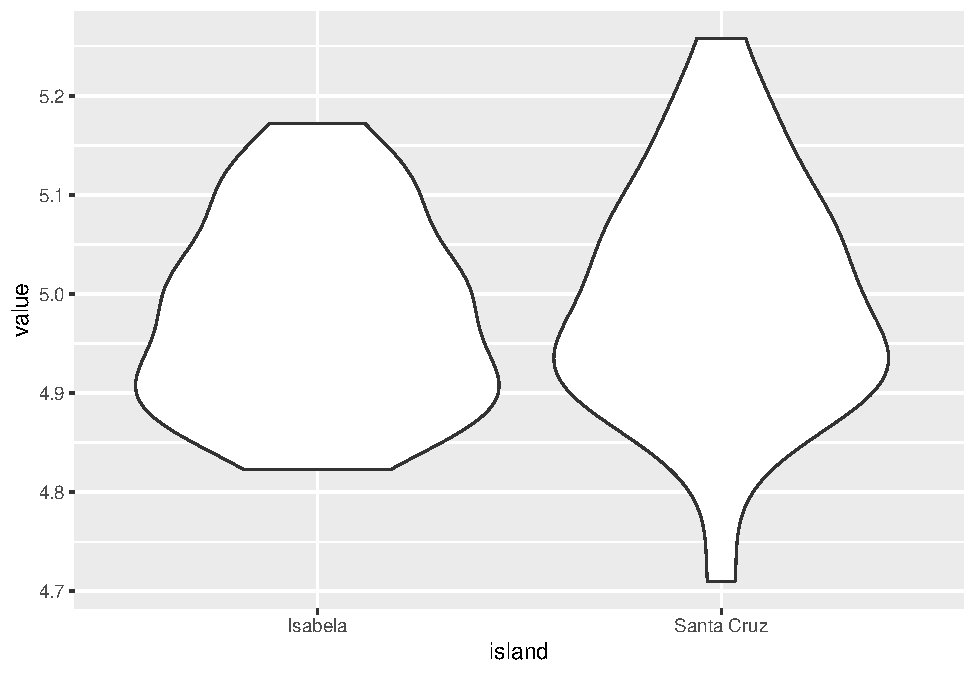
\includegraphics{TRES-Tidy-Tutorial_files/figure-latex/unnamed-chunk-55-1.pdf}

We could use factor reordering to change the order of the violins:

\begin{Shaded}
\begin{Highlighting}[]
\NormalTok{data}\OperatorTok{$}\NormalTok{island <-}\StringTok{ }\KeywordTok{fct_relevel}\NormalTok{(data}\OperatorTok{$}\NormalTok{island, }\KeywordTok{c}\NormalTok{(}\StringTok{"Santa Cruz"}\NormalTok{, }\StringTok{"Isabela"}\NormalTok{))}
\KeywordTok{ggplot}\NormalTok{(data[data}\OperatorTok{$}\NormalTok{variable }\OperatorTok{==}\StringTok{ "beak_length"}\NormalTok{,], }\KeywordTok{aes}\NormalTok{(}\DataTypeTok{x =}\NormalTok{ island, }\DataTypeTok{y =}\NormalTok{ value)) }\OperatorTok{+}
\StringTok{  }\KeywordTok{geom_violin}\NormalTok{()}
\end{Highlighting}
\end{Shaded}

\begin{verbatim}
## Warning: Removed 36 rows containing non-finite values (stat_ydensity).
\end{verbatim}

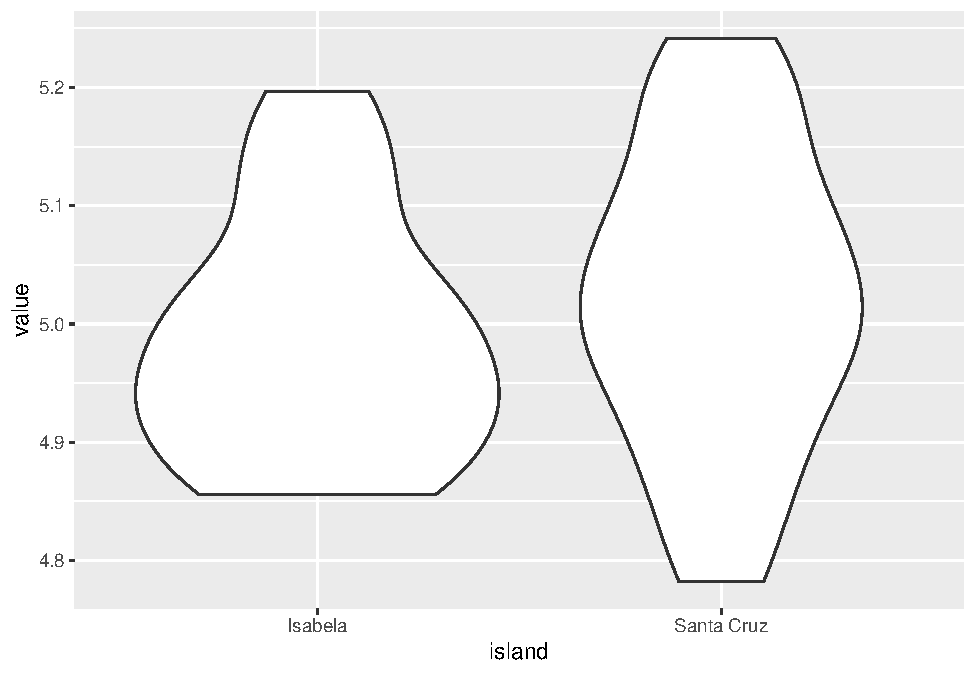
\includegraphics{TRES-Tidy-Tutorial_files/figure-latex/unnamed-chunk-56-1.pdf}

Lots of other variants exist for reordering (e.g.~reordering by association with a variable), which we do not cover here. Please refer to the \href{https://rstudio.com/resources/cheatsheets/}{cheatsheet} or the online documentation for more examples.

\hypertarget{factor-levels}{%
\subsection{4.2. Factor levels}\label{factor-levels}}

One can change the levels of a factor using \texttt{fct\_recode}:

\begin{Shaded}
\begin{Highlighting}[]
\KeywordTok{fct_recode}\NormalTok{(}
\NormalTok{  my_fact_vec, }
  \StringTok{"Pratik Gupte"}\NormalTok{ =}\StringTok{ "Pratik"}\NormalTok{, }
  \StringTok{"Theo Pannetier"}\NormalTok{ =}\StringTok{ "Theo"}\NormalTok{, }
  \StringTok{"Raphael Scherrer"}\NormalTok{ =}\StringTok{ "Raph"}
\NormalTok{)}
\end{Highlighting}
\end{Shaded}

\begin{verbatim}
## [1] Pratik Gupte     Theo Pannetier   Raphael Scherrer
## Levels: Pratik Gupte Raphael Scherrer Theo Pannetier
\end{verbatim}

or collapse factor levels together using \texttt{fct\_collapse}:

\begin{Shaded}
\begin{Highlighting}[]
\KeywordTok{fct_collapse}\NormalTok{(my_fact_vec, }\DataTypeTok{EU =} \KeywordTok{c}\NormalTok{(}\StringTok{"Theo"}\NormalTok{, }\StringTok{"Raph"}\NormalTok{), }\DataTypeTok{NonEU =} \StringTok{"Pratik"}\NormalTok{)}
\end{Highlighting}
\end{Shaded}

\begin{verbatim}
## [1] NonEU EU    EU   
## Levels: NonEU EU
\end{verbatim}

Again, we do not provide an exhaustive list of \texttt{forcats} functions here but the most usual ones, to give a glimpse of many things that one can do with factors. So, if you are dealing with factors, remember that \texttt{forcats} may have handy tools for you.

\hypertarget{bonus-dropping-levels}{%
\subsection{4.3. Bonus: dropping levels}\label{bonus-dropping-levels}}

If you use factors in your tibble and get rid of one level, for any reason, the factor will usually remember the old levels, which may cause some problems when applying functions to your data.

\begin{Shaded}
\begin{Highlighting}[]
\NormalTok{data <-}\StringTok{ }\NormalTok{data[data}\OperatorTok{$}\NormalTok{island }\OperatorTok{==}\StringTok{ "Santa Cruz"}\NormalTok{,]}
\KeywordTok{unique}\NormalTok{(data}\OperatorTok{$}\NormalTok{island) }\CommentTok{# Isabela is gone from the labels}
\end{Highlighting}
\end{Shaded}

\begin{verbatim}
## [1] Santa Cruz
## Levels: Santa Cruz Isabela
\end{verbatim}

\begin{Shaded}
\begin{Highlighting}[]
\KeywordTok{levels}\NormalTok{(data}\OperatorTok{$}\NormalTok{island) }\CommentTok{# but not from the levels}
\end{Highlighting}
\end{Shaded}

\begin{verbatim}
## [1] "Santa Cruz" "Isabela"
\end{verbatim}

Use \texttt{droplevels} (from base R) to make sure you get rid of levels that are not in your data anymore:

\begin{Shaded}
\begin{Highlighting}[]
\NormalTok{data <-}\StringTok{ }\KeywordTok{droplevels}\NormalTok{(data)}
\KeywordTok{levels}\NormalTok{(data}\OperatorTok{$}\NormalTok{island)}
\end{Highlighting}
\end{Shaded}

\begin{verbatim}
## [1] "Santa Cruz"
\end{verbatim}

Fortunately, most functions within the tidyverse will not complain about missing levels, and will automatically get rid of those inexistant levels for you. But because factors are such common causes of bugs, keep this in mind!

\hypertarget{external-resources}{%
\section{5. External resources}\label{external-resources}}

Find lots of additional info by looking up the following links:

\begin{itemize}
\tightlist
\item
  The \texttt{readr}/\texttt{tibble}/\texttt{tidyr} and \texttt{forcats} \href{https://rstudio.com/resources/cheatsheets/}{cheatsheets}.
\item
  This \href{https://tidyr.tidyverse.org/articles/tidy-data.html}{link} on the concept of tidy data
\item
  The \href{https://tibble.tidyverse.org/}{tibble}, \href{https://tidyr.tidyverse.org/}{tidyr} and \href{https://forcats.tidyverse.org/}{forcats} websites
\end{itemize}

\hypertarget{data-manipulation-with-dplyr}{%
\chapter{\texorpdfstring{Data manipulation with \texttt{dplyr}}{Data manipulation with dplyr}}\label{data-manipulation-with-dplyr}}

\begin{Shaded}
\begin{Highlighting}[]
\CommentTok{# load the tidyverse}
\KeywordTok{library}\NormalTok{(tidyverse)}
\end{Highlighting}
\end{Shaded}

\begin{verbatim}
## -- Attaching packages --------------------------------------- tidyverse 1.3.0 --
\end{verbatim}

\begin{verbatim}
## v purrr 0.3.4     v dplyr 0.8.5
\end{verbatim}

\begin{verbatim}
## -- Conflicts ------------------------------------------ tidyverse_conflicts() --
## x dplyr::collapse() masks glue::collapse()
## x dplyr::filter()   masks stats::filter()
## x dplyr::lag()      masks stats::lag()
\end{verbatim}

\hypertarget{introduction}{%
\section{Introduction}\label{introduction}}

Reminders from last weeks: pipe operator, tidy tables, ggplot

Why dplyr ? dplyr vs base R

\hypertarget{example-data-of-the-day}{%
\section{Example data of the day}\label{example-data-of-the-day}}

Through this tutorial, we will be using mammal trait data from the \href{https://megapast2future.github.io/PHYLACINE_1.2/}{Phylacine} database. The dataset contains information on mass, diet, life habit, etc, for more than all living species of mammals. Let's have a look.

\begin{Shaded}
\begin{Highlighting}[]
\NormalTok{phylacine <-}\StringTok{ }\NormalTok{readr}\OperatorTok{::}\KeywordTok{read_csv}\NormalTok{(}\StringTok{"data/phylacine_traits.csv"}\NormalTok{)}
\NormalTok{phylacine}
\end{Highlighting}
\end{Shaded}

\begin{verbatim}
## # A tibble: 5,831 x 24
##    Binomial.1.2 Order.1.2 Family.1.2 Genus.1.2 Species.1.2 Terrestrial Marine
##    <chr>        <chr>     <chr>      <chr>     <chr>             <dbl>  <dbl>
##  1 Abditomys_l~ Rodentia  Muridae    Abditomys latidens              1      0
##  2 Abeomelomys~ Rodentia  Muridae    Abeomelo~ sevia                 1      0
##  3 Abrawayaomy~ Rodentia  Cricetidae Abrawaya~ ruschii               1      0
##  4 Abrocoma_be~ Rodentia  Abrocomid~ Abrocoma  bennettii             1      0
##  5 Abrocoma_bo~ Rodentia  Abrocomid~ Abrocoma  boliviensis           1      0
##  6 Abrocoma_bu~ Rodentia  Abrocomid~ Abrocoma  budini                1      0
##  7 Abrocoma_ci~ Rodentia  Abrocomid~ Abrocoma  cinerea               1      0
##  8 Abrocoma_fa~ Rodentia  Abrocomid~ Abrocoma  famatina              1      0
##  9 Abrocoma_sh~ Rodentia  Abrocomid~ Abrocoma  shistacea             1      0
## 10 Abrocoma_us~ Rodentia  Abrocomid~ Abrocoma  uspallata             1      0
## # ... with 5,821 more rows, and 17 more variables: Freshwater <dbl>,
## #   Aerial <dbl>, Life.Habit.Method <chr>, Life.Habit.Source <chr>,
## #   Mass.g <dbl>, Mass.Method <chr>, Mass.Source <chr>, Mass.Comparison <chr>,
## #   Mass.Comparison.Source <chr>, Island.Endemicity <chr>,
## #   IUCN.Status.1.2 <chr>, Added.IUCN.Status.1.2 <chr>, Diet.Plant <dbl>,
## #   Diet.Vertebrate <dbl>, Diet.Invertebrate <dbl>, Diet.Method <chr>,
## #   Diet.Source <chr>
\end{verbatim}

Note the friendly output given by the \texttt{tibble} (as opposed to a \texttt{data.frame}). \texttt{readr} automatically stores the content it reads in a \texttt{tibble}, tidyverse oblige. You should know however that \texttt{dplyr} doesn't require your data to be in a tibble, a regular \texttt{data.frame} will work just as fine.

Most of the \texttt{dplyr} verbs covered in the next sections assume your data is \emph{tidy}: wide format, variables as column, 1 observation per row. Not that tehy won't work if your data isn't tidy, but the results could be very different from what I'm going to show here. Fortunately, the phylacine trait dataset appears to be tidy: there is one unique entry for each species.

The first operation I'm going to run on this table is changing the names with
\texttt{rename()}. Some people prefer their tea without sugar, and I \href{https://style.tidyverse.org/syntax.html\#object-names}{prefer} my
variable names without uppercase characters, dots or (if possible) numbers.
This will give me the opportunity to introduce the trivial syntax
of \texttt{dplyr} verbs.

\begin{Shaded}
\begin{Highlighting}[]
\NormalTok{phylacine <-}\StringTok{ }\NormalTok{phylacine }\OperatorTok\StringTok{ }
\StringTok{  }\NormalTok{dplyr}\OperatorTok{::}\KeywordTok{rename}\NormalTok{(}
    \StringTok{"binomial"}\NormalTok{ =}\StringTok{ }\NormalTok{Binomial.}\FloatTok{1.2}\NormalTok{,}
    \StringTok{"order"}\NormalTok{ =}\StringTok{ }\NormalTok{Order.}\FloatTok{1.2}\NormalTok{,}
    \StringTok{"family"}\NormalTok{ =}\StringTok{ }\NormalTok{Family.}\FloatTok{1.2}\NormalTok{,}
    \StringTok{"genus"}\NormalTok{ =}\StringTok{ }\NormalTok{Genus.}\FloatTok{1.2}\NormalTok{,}
    \StringTok{"species"}\NormalTok{ =}\StringTok{ }\NormalTok{Species.}\FloatTok{1.2}\NormalTok{,}
    \StringTok{"terrestrial"}\NormalTok{ =}\StringTok{ }\NormalTok{Terrestrial,}
    \StringTok{"marine"}\NormalTok{ =}\StringTok{ }\NormalTok{Marine,}
    \StringTok{"freshwater"}\NormalTok{ =}\StringTok{ }\NormalTok{Freshwater,}
    \StringTok{"aerial"}\NormalTok{ =}\StringTok{ }\NormalTok{Aerial,}
    \StringTok{"life_habit_method"}\NormalTok{ =}\StringTok{ }\NormalTok{Life.Habit.Method,}
    \StringTok{"life_habit_source"}\NormalTok{ =}\StringTok{ }\NormalTok{Life.Habit.Source,}
    \StringTok{"mass_g"}\NormalTok{ =}\StringTok{ }\NormalTok{Mass.g,}
    \StringTok{"mass_method"}\NormalTok{ =}\StringTok{ }\NormalTok{Mass.Method,}
    \StringTok{"mass_source"}\NormalTok{ =}\StringTok{ }\NormalTok{Mass.Source,}
    \StringTok{"mass_comparison"}\NormalTok{ =}\StringTok{ }\NormalTok{Mass.Comparison,}
    \StringTok{"mass_comparison_source"}\NormalTok{ =}\StringTok{ }\NormalTok{Mass.Comparison.Source,}
    \StringTok{"island_endemicity"}\NormalTok{ =}\StringTok{ }\NormalTok{Island.Endemicity,}
    \StringTok{"iucn_status"}\NormalTok{ =}\StringTok{ }\NormalTok{IUCN.Status.}\FloatTok{1.2}\NormalTok{, }\CommentTok{# not even for acronyms}
    \StringTok{"added_iucn_status"}\NormalTok{ =}\StringTok{  }\NormalTok{Added.IUCN.Status.}\FloatTok{1.2}\NormalTok{,}
    \StringTok{"diet_plant"}\NormalTok{ =}\StringTok{ }\NormalTok{Diet.Plant,}
    \StringTok{"diet_vertebrate"}\NormalTok{ =}\StringTok{ }\NormalTok{Diet.Vertebrate,}
    \StringTok{"diet_invertebrate"}\NormalTok{ =}\StringTok{ }\NormalTok{Diet.Invertebrate,}
    \StringTok{"diet_method"}\NormalTok{ =}\StringTok{ }\NormalTok{Diet.Method,}
    \StringTok{"diet_source"}\NormalTok{ =}\StringTok{ }\NormalTok{Diet.Source}
\NormalTok{  )}
\end{Highlighting}
\end{Shaded}

For convenience, I'm going to use the pipe operator (\texttt{\%\textgreater{}\%}) that we've seen
before, through this chapter. All \texttt{dplyr} functions are built to work with the
pipe (i.e, their firstargument is always \texttt{data}), but again, this is not
compulsory. I could do

\begin{Shaded}
\begin{Highlighting}[]
\NormalTok{phylacine <-}\StringTok{ }\NormalTok{dplyr}\OperatorTok{::}\KeywordTok{rename}\NormalTok{(}
  \DataTypeTok{data =}\NormalTok{ phylacine,}
  \StringTok{"binomial"}\NormalTok{ =}\StringTok{ }\NormalTok{Binomial.}\FloatTok{1.2}\NormalTok{,}
  \CommentTok{# ...}
\NormalTok{)}
\end{Highlighting}
\end{Shaded}

Note how columns are referred to. Once the data as been passed as an argument,
no need to refer to it anymore, \texttt{dplyr} understands that you're dealing with
variables inside that data frame. So drop that \texttt{data\$var}, \texttt{data{[},\ "var"{]}},
and, if you've read \emph{The R book}, forget the very existence of \texttt{attach()}.

Finally, I should mention that you can refer to variables names either with strings or directly as objects, whether you're reading or creating them:

\begin{Shaded}
\begin{Highlighting}[]
\NormalTok{phylacine2 <-}\StringTok{ }\NormalTok{readr}\OperatorTok{::}\KeywordTok{read_csv}\NormalTok{(}\StringTok{"data/phylacine_traits.csv"}\NormalTok{)}

\NormalTok{phylacine2 }\OperatorTok\StringTok{ }
\StringTok{  }\NormalTok{dplyr}\OperatorTok{::}\KeywordTok{rename}\NormalTok{(}
    \CommentTok{# this works}
    \DataTypeTok{binomial =}\NormalTok{ Binomial.}\FloatTok{1.2}
\NormalTok{  )}
\NormalTok{phylacine2 }\OperatorTok\StringTok{ }
\StringTok{  }\NormalTok{dplyr}\OperatorTok{::}\KeywordTok{rename}\NormalTok{(}
    \CommentTok{# this works too!}
    \DataTypeTok{binomial =} \StringTok{"Binomial.1.2"}
\NormalTok{  )}
\NormalTok{phylacine2 }\OperatorTok\StringTok{ }
\StringTok{  }\NormalTok{dplyr}\OperatorTok{::}\KeywordTok{rename}\NormalTok{(}
    \CommentTok{# guess what}
    \StringTok{"binomial"}\NormalTok{ =}\StringTok{ "Binomial.1.2"}
\NormalTok{  )}
\end{Highlighting}
\end{Shaded}

\hypertarget{select-variables-with-select}{%
\section{\texorpdfstring{Select variables with \texttt{select()}}{Select variables with select()}}\label{select-variables-with-select}}

\hypertarget{select-observations-with-filter}{%
\section{\texorpdfstring{Select observations with \texttt{filter()}}{Select observations with filter()}}\label{select-observations-with-filter}}

\hypertarget{create-new-variables-with-mutate}{%
\section{\texorpdfstring{Create new variables with \texttt{mutate()}}{Create new variables with mutate()}}\label{create-new-variables-with-mutate}}

can also edit existing ones

drop existing variables with \texttt{transmute()}

\hypertarget{grouped-results-with-group_by-and-summarise}{%
\section{\texorpdfstring{Grouped results with \texttt{group\_by()} and \texttt{summarise()}}{Grouped results with group\_by() and summarise()}}\label{grouped-results-with-group_by-and-summarise}}

\hypertarget{scoped-variables}{%
\section{Scoped variables}\label{scoped-variables}}

\begin{Shaded}
\begin{Highlighting}[]
\KeywordTok{data}\NormalTok{(mtcars)}
\NormalTok{mtcars }\OperatorTok\StringTok{ }\KeywordTok{select_all}\NormalTok{(toupper)}

\NormalTok{is_whole <-}\StringTok{ }\ControlFlowTok{function}\NormalTok{(x) }\KeywordTok{all}\NormalTok{(}\KeywordTok{floor}\NormalTok{(x) }\OperatorTok{==}\StringTok{ }\NormalTok{x)}
\NormalTok{mtcars }\OperatorTok\StringTok{ }\KeywordTok{select_if}\NormalTok{() }\CommentTok{# select integers only}

\NormalTok{mtcars }\OperatorTok\StringTok{ }\KeywordTok{select_at}\NormalTok{(}\KeywordTok{vars}\NormalTok{(}\OperatorTok{-}\KeywordTok{contains}\NormalTok{(}\StringTok{"ar"}\NormalTok{)))}
\NormalTok{mtcars }\OperatorTok\StringTok{ }\KeywordTok{select_at}\NormalTok{(}\KeywordTok{vars}\NormalTok{(}\OperatorTok{-}\KeywordTok{contains}\NormalTok{(}\StringTok{"ar"}\NormalTok{), }\KeywordTok{starts_with}\NormalTok{(}\StringTok{"c"}\NormalTok{)))}
\end{Highlighting}
\end{Shaded}

\hypertarget{more}{%
\section{More !}\label{more}}

dolla sign x point operator
variables values -\textgreater{} dplyr::distinct() eq. to base::unique()
sample()
slice()

\hypertarget{working-with-lists-and-iteration}{%
\chapter{Working with lists and iteration}\label{working-with-lists-and-iteration}}


\includegraphics{opening-image.png}

\begin{Shaded}
\begin{Highlighting}[]
\CommentTok{# load the tidyverse}
\KeywordTok{library}\NormalTok{(tidyverse)}
\end{Highlighting}
\end{Shaded}

\hypertarget{basic-iteration-with-map}{%
\section{\texorpdfstring{Basic iteration with \texttt{map}}{Basic iteration with map}}\label{basic-iteration-with-map}}

Iteration in base \texttt{R} is commonly done with \texttt{for} and \texttt{while} loops.
There is no readymade alternative to \texttt{while} loops in the tidyverse.
However, the functionality of \texttt{for} loops is spread over the \texttt{map} family of functions.

\texttt{purrr} functions are \emph{functionals}, i.e., functions that take another function as an argument.
The closest equivalent in \texttt{R} is the \texttt{*apply} family of functions: \texttt{apply}, \texttt{lapply}, \texttt{vapply} and so on.

A good reason to use \texttt{purrr} functions instead of base \texttt{R} functions is their consistent and clear naming, which always indicates how they should be used.
This is explained in the examples below.

These reasons, as well as how \texttt{map} is different from \texttt{for} and \texttt{lapply} are best explained in the \href{https://adv-r.hadley.nz/functionals.html}{Advanced R book}.

\hypertarget{map-basic-use}{%
\subsection{\texorpdfstring{\texttt{map} basic use}{map basic use}}\label{map-basic-use}}

\texttt{map} works on any list-like object, which includes vectors, and always returns a list. \texttt{map} takes two arguments, the object on which to operate, and the function to apply to each element.

\begin{Shaded}
\begin{Highlighting}[]
\CommentTok{# get the square root of each integer 1 - 10}
\NormalTok{some_numbers =}\StringTok{ }\DecValTok{1}\OperatorTok{:}\DecValTok{10}
\KeywordTok{map}\NormalTok{(some_numbers, sqrt)}
\end{Highlighting}
\end{Shaded}

\begin{verbatim}
## [[1]]
## [1] 1
## 
## [[2]]
## [1] 1.414214
## 
## [[3]]
## [1] 1.732051
## 
## [[4]]
## [1] 2
## 
## [[5]]
## [1] 2.236068
## 
## [[6]]
## [1] 2.44949
## 
## [[7]]
## [1] 2.645751
## 
## [[8]]
## [1] 2.828427
## 
## [[9]]
## [1] 3
## 
## [[10]]
## [1] 3.162278
\end{verbatim}

\hypertarget{map-variants-returning-vectors}{%
\subsection{\texorpdfstring{\texttt{map} variants returning vectors}{map variants returning vectors}}\label{map-variants-returning-vectors}}

Though \texttt{map} always returns a list, it has variants named \texttt{map\_*} where the suffix indicates the return type.
\texttt{map\_chr}, \texttt{map\_dbl}, \texttt{map\_int}, and \texttt{map\_lgl} return character, double (numeric), integer, and logical vectors.

\begin{Shaded}
\begin{Highlighting}[]
\CommentTok{# use map_dbl to get a vector of square roots}
\NormalTok{some_numbers =}\StringTok{ }\DecValTok{1}\OperatorTok{:}\DecValTok{10}
\KeywordTok{map_dbl}\NormalTok{(some_numbers, sqrt)}
\end{Highlighting}
\end{Shaded}

\begin{verbatim}
##  [1] 1.000000 1.414214 1.732051 2.000000 2.236068 2.449490 2.645751 2.828427
##  [9] 3.000000 3.162278
\end{verbatim}

\begin{Shaded}
\begin{Highlighting}[]
\CommentTok{# map_chr will convert the output to a character}
\KeywordTok{map_chr}\NormalTok{(some_numbers, sqrt)}
\end{Highlighting}
\end{Shaded}

\begin{verbatim}
##  [1] "1.000000" "1.414214" "1.732051" "2.000000" "2.236068" "2.449490"
##  [7] "2.645751" "2.828427" "3.000000" "3.162278"
\end{verbatim}

\begin{Shaded}
\begin{Highlighting}[]
\CommentTok{# map_int will NOT round the output to an integer}

\CommentTok{# map_lgl returns TRUE/FALSE values}
\NormalTok{some_numbers =}\StringTok{ }\KeywordTok{c}\NormalTok{(}\OtherTok{NA}\NormalTok{, }\DecValTok{1}\OperatorTok{:}\DecValTok{3}\NormalTok{, }\OtherTok{NA}\NormalTok{, }\OtherTok{NaN}\NormalTok{, }\OtherTok{Inf}\NormalTok{, }\OperatorTok{-}\OtherTok{Inf}\NormalTok{)}
\KeywordTok{map_lgl}\NormalTok{(some_numbers, is.na)}
\end{Highlighting}
\end{Shaded}

\begin{verbatim}
## [1]  TRUE FALSE FALSE FALSE  TRUE  TRUE FALSE FALSE
\end{verbatim}

\hypertarget{integrating-map-and-tidyrnest}{%
\subsection*{\texorpdfstring{Integrating \texttt{map} and \texttt{tidyr::nest}}{Integrating map and tidyr::nest}}\label{integrating-map-and-tidyrnest}}
\addcontentsline{toc}{subsection}{Integrating \texttt{map} and \texttt{tidyr::nest}}

The example show how each map variant can be used. This integrates \texttt{tidyr::nest} with \texttt{map}, and the two are especially complementary.

\begin{Shaded}
\begin{Highlighting}[]
\CommentTok{# nest mtcars into a list of dataframes based on number of cylinders}
\NormalTok{some_data =}\StringTok{ }\KeywordTok{as_tibble}\NormalTok{(mtcars, }\DataTypeTok{rownames =} \StringTok{"car_name"}\NormalTok{) }\OperatorTok\StringTok{ }
\StringTok{  }\KeywordTok{group_by}\NormalTok{(cyl) }\OperatorTok\StringTok{ }
\StringTok{  }\KeywordTok{nest}\NormalTok{()}

\CommentTok{# get the number of rows per dataframe}
\CommentTok{# the mean mileage}
\CommentTok{# and the first car}
\NormalTok{some_data =}\StringTok{ }\NormalTok{some_data }\OperatorTok\StringTok{ }
\StringTok{  }\KeywordTok{mutate}\NormalTok{(}\DataTypeTok{n_rows =} \KeywordTok{map_int}\NormalTok{(data, nrow),}
         \DataTypeTok{mean_mpg =} \KeywordTok{map_dbl}\NormalTok{(data, }\OperatorTok{~}\KeywordTok{mean}\NormalTok{(.}\OperatorTok{$}\NormalTok{mpg)),}
         \DataTypeTok{first_car =} \KeywordTok{map_chr}\NormalTok{(data, }\OperatorTok{~}\KeywordTok{first}\NormalTok{(.}\OperatorTok{$}\NormalTok{car_name)))}

\NormalTok{some_data}
\end{Highlighting}
\end{Shaded}

\begin{verbatim}
## # A tibble: 3 x 5
## # Groups:   cyl [3]
##     cyl data               n_rows mean_mpg first_car        
##   <dbl> <list>              <int>    <dbl> <chr>            
## 1     6 <tibble [7 x 11]>       7     19.7 Mazda RX4        
## 2     4 <tibble [11 x 11]>     11     26.7 Datsun 710       
## 3     8 <tibble [14 x 11]>     14     15.1 Hornet Sportabout
\end{verbatim}

\texttt{map} accepts multiple functions that are applied in sequence to the input list-like object, but this is confusing to the reader and ill advised.

\hypertarget{map-variants-returning-dataframes}{%
\subsection{\texorpdfstring{\texttt{map} variants returning dataframes}{map variants returning dataframes}}\label{map-variants-returning-dataframes}}

\texttt{map\_df} returns data frames, and by default binds dataframes by rows, while \texttt{map\_dfr} does this explicitly, and \texttt{map\_dfc} does returns a dataframe bound by column.

\begin{Shaded}
\begin{Highlighting}[]
\CommentTok{# split mtcars into 3 dataframes, one per cylinder number}
\NormalTok{some_list =}\StringTok{ }\KeywordTok{split}\NormalTok{(mtcars, mtcars}\OperatorTok{$}\NormalTok{cyl)}

\CommentTok{# get the first two rows of each dataframe}
\KeywordTok{map_df}\NormalTok{(some_list, head, }\DataTypeTok{n =} \DecValTok{2}\NormalTok{)}
\end{Highlighting}
\end{Shaded}

\begin{verbatim}
##    mpg cyl  disp  hp drat    wt  qsec vs am gear carb
## 1 22.8   4 108.0  93 3.85 2.320 18.61  1  1    4    1
## 2 24.4   4 146.7  62 3.69 3.190 20.00  1  0    4    2
## 3 21.0   6 160.0 110 3.90 2.620 16.46  0  1    4    4
## 4 21.0   6 160.0 110 3.90 2.875 17.02  0  1    4    4
## 5 18.7   8 360.0 175 3.15 3.440 17.02  0  0    3    2
## 6 14.3   8 360.0 245 3.21 3.570 15.84  0  0    3    4
\end{verbatim}

\texttt{map} accepts arguments to the function being mapped, such as in the example above, where \texttt{head()} accepts the argument \texttt{n\ =\ 2}.

\texttt{map\_dfr} behaves the same as \texttt{map\_df}.

\begin{Shaded}
\begin{Highlighting}[]
\CommentTok{# the same as above but with a pipe}
\NormalTok{some_list }\OperatorTok\StringTok{ }
\StringTok{  }\KeywordTok{map_dfr}\NormalTok{(head, }\DataTypeTok{n =} \DecValTok{2}\NormalTok{)}
\end{Highlighting}
\end{Shaded}

\begin{verbatim}
##    mpg cyl  disp  hp drat    wt  qsec vs am gear carb
## 1 22.8   4 108.0  93 3.85 2.320 18.61  1  1    4    1
## 2 24.4   4 146.7  62 3.69 3.190 20.00  1  0    4    2
## 3 21.0   6 160.0 110 3.90 2.620 16.46  0  1    4    4
## 4 21.0   6 160.0 110 3.90 2.875 17.02  0  1    4    4
## 5 18.7   8 360.0 175 3.15 3.440 17.02  0  0    3    2
## 6 14.3   8 360.0 245 3.21 3.570 15.84  0  0    3    4
\end{verbatim}

\texttt{map\_dfc} binds the resulting 3 data frames of two rows each by column, and automatically repairs the column names, adding a suffix to each duplicate.

\begin{Shaded}
\begin{Highlighting}[]
\NormalTok{some_list }\OperatorTok\StringTok{ }
\StringTok{  }\KeywordTok{map_dfc}\NormalTok{(head, }\DataTypeTok{n =} \DecValTok{2}\NormalTok{)}
\end{Highlighting}
\end{Shaded}

\begin{verbatim}
##    mpg cyl  disp hp drat   wt  qsec vs am gear carb mpg1 cyl1 disp1 hp1 drat1
## 1 22.8   4 108.0 93 3.85 2.32 18.61  1  1    4    1   21    6   160 110   3.9
## 2 24.4   4 146.7 62 3.69 3.19 20.00  1  0    4    2   21    6   160 110   3.9
##     wt1 qsec1 vs1 am1 gear1 carb1 mpg2 cyl2 disp2 hp2 drat2  wt2 qsec2 vs2 am2
## 1 2.620 16.46   0   1     4     4 18.7    8   360 175  3.15 3.44 17.02   0   0
## 2 2.875 17.02   0   1     4     4 14.3    8   360 245  3.21 3.57 15.84   0   0
##   gear2 carb2
## 1     3     2
## 2     3     4
\end{verbatim}

\hypertarget{selective-mapping}{%
\subsection{Selective mapping}\label{selective-mapping}}

\begin{itemize}
\tightlist
\item
  \texttt{map\_at} and \texttt{map\_if}
\end{itemize}

\hypertarget{more-map-variants}{%
\section{\texorpdfstring{More \texttt{map} variants}{More map variants}}\label{more-map-variants}}

\hypertarget{map2}{%
\subsection{\texorpdfstring{\texttt{map2}}{map2}}\label{map2}}

\texttt{imap} here

\hypertarget{pmap}{%
\subsection{\texorpdfstring{\texttt{pmap}}{pmap}}\label{pmap}}

\hypertarget{walk}{%
\subsection{\texorpdfstring{\texttt{walk}}{walk}}\label{walk}}

\texttt{walk2} and \texttt{pwalk}

\hypertarget{modification-in-place}{%
\section{Modification in place}\label{modification-in-place}}

\texttt{modify}

\hypertarget{working-with-lists}{%
\section{Working with lists}\label{working-with-lists}}

\hypertarget{filtering-lists}{%
\subsection{Filtering lists}\label{filtering-lists}}

\hypertarget{summarising-lists}{%
\subsection{Summarising lists}\label{summarising-lists}}

\hypertarget{reduction-and-accumulation}{%
\subsection{Reduction and accumulation}\label{reduction-and-accumulation}}

\hypertarget{miscellaneous-operation}{%
\subsection{Miscellaneous operation}\label{miscellaneous-operation}}

\end{document}
